% =============================================================
%  Design and Implementation of an AI-Driven Orchestration
%  and Decision System for Automated Penetration Testing
%
%  The Phantom System --- PFE Master Thesis
%  Author     : Rodwan Gadouri  <r_gadouri@estin.dz>
%  Supervisor : Dr. Allama Oussama
%  ESTIN, Bejaia, Algeria --- Academic Year 2025--2026
%
%  BEAUTIFIED VERSION (Matching thesis_beautiful.tex)
%  - A4, Times New Roman 12pt, 1.5 spacing, standard paragraph indents
%  - Asymmetrical geometry for binding (left=3cm, right=2.5cm)
%  - Language: English
%  - Bibliography: APA (biblatex)
%  - Verification: all architectural claims traced to source file:line
% =============================================================
\documentclass[12pt, a4paper, oneside, openany]{book}

%% === FONTS (Times Roman from thesis_beautiful) =================
\usepackage[T1]{fontenc}
\usepackage[utf8]{inputenc}
\usepackage{mathptmx}
\usepackage{amsmath}
\usepackage{amssymb}

%% === PAGE GEOMETRY (From thesis_beautiful.tex) ===============
\usepackage[top=2.5cm,bottom=2.5cm,left=3cm,right=2.5cm]{geometry}

%% === HEAD HEIGHT (fancyhdr requires ≥14pt for running headers)
\setlength{\headheight}{14pt}

%% === LINE SPACING (From thesis_beautiful.tex) ======
\usepackage{setspace}
\onehalfspacing

\hbadness=10000
\vbadness=10000

%% === COLORS =================================================
\usepackage{xcolor}
\definecolor{navy}{RGB}{0,0,128}
\definecolor{darkblue}{RGB}{0,51,102}
\definecolor{headercolor}{RGB}{51,102,153}
\definecolor{lightgray}{RGB}{240,240,240}
\definecolor{phantomblue}{RGB}{30,90,180}
\definecolor{critred}{RGB}{190,30,30}
\definecolor{highorg}{RGB}{210,110,20}
\definecolor{lowgrn}{RGB}{40,140,40}
\definecolor{codebg}{RGB}{247,247,252}
\definecolor{rowalt}{RGB}{248,251,255}
\definecolor{layerA}{RGB}{230,240,255}
\definecolor{layerB}{RGB}{230,255,235}
\definecolor{layerC}{RGB}{255,245,220}
\definecolor{layerD}{RGB}{255,230,230}
\definecolor{tabhead}{RGB}{20,60,120}

%% === HEADER / FOOTER ========================================
\usepackage{fancyhdr}
\pagestyle{fancy}
\fancyhf{}

\renewcommand{\chaptermark}[1]{%
  \ifnum\value{chapter}>0
    \markboth{Chapter \thechapter:\ #1}{}%
  \else
    \markboth{#1}{}%
  \fi
}
\renewcommand{\sectionmark}[1]{}

\fancyhead[L]{\nouppercase{\leftmark}}
\fancyfoot[C]{}
\fancyfoot[R]{\thepage}

\fancypagestyle{plain}{%
  \fancyhf{}%
  \fancyfoot[R]{\thepage}%
  \renewcommand{\headrulewidth}{0pt}}

%% === CHAPTER & SECTION HEADINGS =============================
\usepackage{titlesec}
\titleformat{\chapter}[block]
  {\normalfont\LARGE\bfseries}
  {Chapter \thechapter}{1em}{\LARGE}

\titleformat{\section}[block]
  {\normalfont\Large\bfseries}
  {\thesection}{1em}{\Large}

\titleformat{\subsection}[block]
  {\normalfont\large\bfseries}
  {\thesubsection}{1em}{\large}

\titleformat{\subsubsection}[hang]
  {\normalfont\normalsize\itshape}
  {\thesubsubsection}{0.6em}{}

\titlespacing{\chapter}{0pt}{2em}{1em}
\titlespacing{\section}{0pt}{1.5em}{0.5em}
\titlespacing{\subsection}{0pt}{1em}{0.3em}
\titlespacing{\subsubsection}{0pt}{6pt}{2pt}

%% === TABLES =================================================
\usepackage{booktabs}
\usepackage{array}
\usepackage{multirow}
\usepackage{tabularx}
\usepackage{colortbl}
\usepackage{longtable}
\newcolumntype{C}[1]{>{\centering\arraybackslash}p{#1}}
\newcolumntype{L}[1]{>{\raggedright\arraybackslash}p{#1}}
\newcolumntype{R}[1]{>{\raggedleft\arraybackslash}p{#1}}

%% === GRAPHICS & CAPTION =====================================
\usepackage{graphicx}
\usepackage{float}
\usepackage{caption}
\captionsetup{font=small, labelfont=bf, labelsep=period,
              justification=justified, singlelinecheck=false}
\usepackage{subcaption}

%% === TikZ ===================================================
\usepackage{tikz}
\usetikzlibrary{
  shapes.geometric, shapes.misc, arrows.meta,
  positioning, fit, backgrounds, calc,
  decorations.pathreplacing, patterns, matrix
}

%% === PGFPLOTS ===============================================
\usepackage{pgfplots}
\pgfplotsset{compat=1.18}

%% === LISTINGS ===============================================
\usepackage{listings}
\lstdefinestyle{phantom}{
  basicstyle=\ttfamily\small,
  backgroundcolor=\color{codebg},
  frame=single, rulecolor=\color{gray!40},
  breaklines=true, breakatwhitespace=true,
  numbers=left, numberstyle=\tiny\color{gray!70},
  numbersep=8pt,
  keywordstyle=\color{phantomblue}\bfseries,
  commentstyle=\color{gray}\itshape,
  stringstyle=\color{critred},
  showstringspaces=false, tabsize=4,
  captionpos=b, xleftmargin=1.5em,
  framexleftmargin=1em,
}
\lstset{style=phantom}

%% === ALGORITHMS =============================================
\usepackage{algorithm}
\usepackage{algpseudocode}
\renewcommand{\algorithmicrequire}{\textbf{Input:}}
\renewcommand{\algorithmicensure}{\textbf{Output:}}

%% === MATH ===================================================
\usepackage{amsmath}
% NOTE: amssymb omitted --- newtxmath already loads it

%% === SYMBOLS ================================================
\usepackage{pifont}
\newcommand{\cmark}{\ding{51}}
\newcommand{\xmk}{\ding{55}}

%% === LISTS ==================================================
\usepackage{enumitem}
\setlist{itemsep=2pt, topsep=4pt}

%% === TCOLORBOX ==============================================
\usepackage{tcolorbox}
\tcbuselibrary{skins, breakable, theorems}

\newtcolorbox{infobox}[1][]{
  enhanced, colback=blue!4, colframe=phantomblue,
  fonttitle=\bfseries\small, title=#1, breakable,
  left=5pt, right=5pt, top=3pt, bottom=3pt,
  attach boxed title to top left={yshift=-2mm, xshift=5mm},
  boxed title style={colback=phantomblue, colframe=phantomblue,
                     fontupper=\color{white}}}

\newtcolorbox{warnbox}[1][]{
  enhanced, colback=red!4, colframe=critred,
  fonttitle=\bfseries\small, title=#1, breakable,
  left=5pt, right=5pt, top=3pt, bottom=3pt,
  attach boxed title to top left={yshift=-2mm, xshift=5mm},
  boxed title style={colback=critred, colframe=critred,
                     fontupper=\color{white}}}

\newtcolorbox{contribbox}[1][]{
  enhanced, colback=lowgrn!5, colframe=lowgrn!70!black,
  fonttitle=\bfseries\small, title=#1, breakable,
  left=5pt, right=5pt, top=3pt, bottom=3pt,
  attach boxed title to top left={yshift=-2mm, xshift=5mm},
  boxed title style={colback=lowgrn!80!black, colframe=lowgrn!80!black,
                     fontupper=\color{white}}}

\newtcolorbox{codebox}[1][]{
  enhanced, colback=codebg, colframe=gray!40,
  fonttitle=\bfseries\small\ttfamily, title=#1, breakable,
  left=5pt, right=5pt, top=3pt, bottom=3pt}

\newtcolorbox{limitbox}[1][]{
  enhanced, colback=highorg!5, colframe=highorg!70!black,
  fonttitle=\bfseries\small, title=#1, breakable,
  left=5pt, right=5pt, top=3pt, bottom=3pt,
  attach boxed title to top left={yshift=-2mm, xshift=5mm},
  boxed title style={colback=highorg!80!black, colframe=highorg!80!black,
                     fontupper=\color{white}}}

%% === BIBLIOGRAPHY ===========================================
\usepackage[backend=biber, style=apa, natbib=true]{biblatex}
\addbibresource{references.bib}

%% === MISC ===================================================
\usepackage{tocbibind}
\usepackage{appendix}

%% === HYPERREF (always last) =================================
\usepackage[pageanchor=false, pdfborder={0 0 0}]{hyperref}
\hypersetup{
  colorlinks=true, linkcolor=black,
  citecolor=black, urlcolor=black,
  pdftitle={Design and Implementation of an AI-Driven Orchestration
            and Decision System for Automated Penetration Testing},
  pdfauthor={Rodwan Gadouri},
  pdfsubject={PFE Master Thesis, ESTIN 2026},
  pdfkeywords={autonomous penetration testing, large language models,
               ReAct, multi-agent, vulnerability detection,
               memory management}}

%% === CUSTOM COMMANDS ========================================
\newcommand{\Phant}{\textit{Phantom}}
\newcommand{\tool}[1]{\texttt{#1}}
\newcommand{\code}[1]{\texttt{#1}}
\newcommand{\file}[1]{\texttt{#1}}

%% === GLOBAL TIKZ STYLES =====================================
\tikzset{
  block/.style={
    rectangle, draw=phantomblue, fill=blue!8,
    text width=2.9cm, minimum height=0.85cm,
    align=center, rounded corners=3pt, font=\small},
  wblock/.style={
    rectangle, draw=phantomblue, fill=blue!8,
    text width=4.8cm, minimum height=0.85cm,
    align=center, rounded corners=3pt, font=\small},
  pstep/.style={
    rectangle, draw=phantomblue, fill=blue!8,
    text width=4.5cm, minimum height=0.82cm,
    align=center, rounded corners=3pt, font=\small},
  decide/.style={
    diamond, draw=highorg, fill=orange!10, aspect=2.1,
    align=center, font=\small, inner sep=1pt},
  phase/.style={
    rectangle, draw=phantomblue, fill=blue!14,
    text width=3.5cm, minimum height=1.1cm,
    align=center, rounded corners=5pt, font=\small\bfseries},
  layer/.style={
    rectangle, draw=phantomblue!50, fill=blue!5,
    text width=13.5cm, minimum height=0.75cm,
    align=center, font=\footnotesize\sffamily, rounded corners=2pt},
  secbox/.style={
    rectangle, draw=critred!60, fill=red!4,
    text width=13.5cm, minimum height=0.75cm,
    align=center, font=\footnotesize\sffamily, rounded corners=2pt},
  cblabel/.style={
    rectangle, draw=phantomblue, fill=blue!14,
    text width=2.3cm, minimum height=0.85cm,
    align=center, rounded corners=6pt, font=\small\bfseries},
  arr/.style={-{Stealth[length=2.5mm]}, thick, phantomblue},
  arrdash/.style={-{Stealth[length=2.5mm]}, thick, dashed, phantomblue!70},
  arrgray/.style={-{Stealth[length=2mm]}, thick, gray!55, dashed},
}

% =============================================================
\begin{document}
% =============================================================

\frontmatter
\pagenumbering{roman}

% ── COVER PAGE ───────────────────────────────────────────────
\thispagestyle{empty}
\begin{titlepage}
\begin{center}
\vspace*{2cm}
{\Huge\bfseries Design and Implementation of an\par}
\vspace{0.5cm}
{\Huge\bfseries AI-Driven Orchestration\par}
\vspace{0.5cm}
{\Huge\bfseries and Decision System\par}
\vspace{2cm}
{\LARGE\bfseries for Automated Penetration Testing\par}
\vspace{3cm}
{\Large MSc Thesis\par}
\vspace{1cm}
{\Large 2026\par}
\vspace{3cm}
\begin{tabular}{c}
{\Large\bfseries Author:} \\[0.3cm]
{\Large Rodwan Gadouri} \\[1cm]
{\Large\bfseries Supervisor:} \\[0.3cm]
{\Large Dr. Allama Oussama}
\end{tabular}
\vfill
\end{center}
\end{titlepage}

\cleardoublepage

% ── DEDICATION ───────────────────────────────────────────────
\chapter*{Dedication}
\addcontentsline{toc}{chapter}{Dedication}

\vspace{1.5cm}
\begin{center}
\textit{To every researcher who reads the source code\\[4pt]
before accepting the documentation.}
\end{center}

\cleardoublepage

% ── ACKNOWLEDGEMENTS ─────────────────────────────────────────
\chapter*{Acknowledgements}
\addcontentsline{toc}{chapter}{Acknowledgements}

I extend my sincere gratitude to my supervisor, Dr.\ Allama Oussama,
whose insistence on verification over assertion shaped the scientific
framing of this work.

I am grateful to the open-source communities behind the OWASP projects,
LiteLLM \citep{litellm2023}, ProjectDiscovery \citep{projectdiscovery_nuclei},
Pydantic~v2, and the broader Python security tooling ecosystem whose
work made the implementation of \Phant{} possible.

\cleardoublepage

% ── ABSTRACT (English) ────────────────────────────────────────
\chapter*{Abstract}
\addcontentsline{toc}{chapter}{Abstract}
\vspace{0.5cm}
\begin{center}
\textbf{\Large Abstract}
\end{center}
\vspace{0.5cm}

Autonomous penetration testing systems must sustain coherent security
reasoning across long-horizon scans while operating under finite context
windows, partial observability, and the risk of process failures.
Signature-based scanners are epistemically bounded by their template
libraries, rendering them structurally incapable of detecting
vulnerability instances absent from those libraries.  Early LLM-based
systems demonstrate reasoning capability but lack the context
management, inter-agent coordination, and crash resilience required
for production-scale deployment.

This thesis presents the design and implementation of \Phant{}, an
open-source autonomous penetration testing system built on the
\textit{ReAct} (Reasoning and Acting) paradigm \citep{yao2023react}.
Four bounded contributions are made: (C1)~a formal description of
the \textit{CVE Template Gap}---the structural detection ceiling of
template-dependent scanners; (C2)~a dual-anchor memory architecture
that aims to preserve critical security findings across context
compression; (C3)~a deterministic hypothesis deduplication mechanism
using exact-match membership over attack surface--vulnerability class
pairs; and (C4)~a code-verified architectural methodology in which
every design claim is traced to a source file and line number,
including the identification of four unreachable subsystems, two
remediated operational bugs (B1, B2), and one live security risk (F6).
No empirical evaluation results are reported; a controlled evaluation
methodology is proposed for future work.

\vspace{0.5cm}
\noindent\textbf{Keywords:} Autonomous Penetration Testing, Large Language Models,
ReAct Paradigm, Multi-Agent Systems, Memory Management, Hypothesis Deduplication.

\cleardoublepage

% ── RÉSUMÉ (French) ──────────────────────────────────────────
\chapter*{R\'{e}sum\'{e}}
\addcontentsline{toc}{chapter}{R\'{e}sum\'{e}}
\vspace{0.5cm}
\begin{center}
\textbf{\Large R\'{e}sum\'{e}}
\end{center}
\vspace{0.5cm}

Les syst\`{e}mes autonomes de test d'intrusion doivent maintenir un
raisonnement de s\'{e}curit\'{e} coh\'{e}rent sur de longues s\'{e}quences
de balayage, tout en op\'{e}rant sous des fen\^{e}tres de contexte finies
et une observabilit\'{e} partielle.  Les scanners \`{a} signatures sont
limit\'{e}s \'{e}pist\'{e}miquement par leurs biblioth\`{e}ques de
mod\`{e}les, ce qui les rend structurellement incapables de d\'{e}tecter
des vuln\'{e}rabilit\'{e}s absentes de ces biblioth\`{e}ques.

Cette th\`{e}se pr\'{e}sente la conception et l'impl\'{e}mentation de
\Phant{}, un syst\`{e}me autonome de test d'intrusion bas\'{e} sur le
paradigme \textit{ReAct}.  Quatre contributions born\'{e}es sont
pr\'{e}sent\'{e}es~: une description formelle du \textit{Foss\'{e} des
Mod\`{e}les CVE}~; une architecture de m\'{e}moire \`{a} double ancrage~;
un m\'{e}canisme de d\'{e}duplication des hypoth\`{e}ses par
correspondance exacte~; et une m\'{e}thodologie architecturale
v\'{e}rifi\'{e}e par le code source.

\vspace{0.5cm}
\noindent\textbf{Mots-cl\'{e}s:} Test d'Intrusion Autonome, Grands
Mod\`{e}les de Langage, Paradigme ReAct, Syst\`{e}mes Multi-Agents,
Gestion de la M\'{e}moire, D\'{e}duplication des Hypoth\`{e}ses.

\cleardoublepage

% ── TABLE OF CONTENTS ────────────────────────────────────────
\tableofcontents
\cleardoublepage

% ── LIST OF FIGURES ──────────────────────────────────────────
\listoffigures
\addcontentsline{toc}{chapter}{List of Figures}
\cleardoublepage

% ── LIST OF TABLES ───────────────────────────────────────────
\listoftables
\addcontentsline{toc}{chapter}{List of Tables}
\cleardoublepage

% ── LIST OF ABBREVIATIONS ────────────────────────────────────
\chapter*{List of Abbreviations}
\addcontentsline{toc}{chapter}{List of Abbreviations}

\begin{tabular}{@{}p{2.2cm}@{}p{10cm}@{}}
\bfseries AI      & Artificial Intelligence \\
\bfseries API     & Application Programming Interface \\
\bfseries CoT     & Chain-of-Thought \\
\bfseries CVE     & Common Vulnerabilities and Exposures \\
\bfseries CVSS    & Common Vulnerability Scoring System \\
\bfseries CWE     & Common Weakness Enumeration \\
\bfseries DAST    & Dynamic Application Security Testing \\
\bfseries DVWA    & Damn Vulnerable Web Application \\
\bfseries FSM     & Finite State Machine \\
\bfseries HMAC    & Hash-based Message Authentication Code \\
\bfseries HTTP    & HyperText Transfer Protocol \\
\bfseries IDOR    & Insecure Direct Object Reference \\
\bfseries LLM     & Large Language Model \\
\bfseries OWASP   & Open Web Application Security Project \\
\bfseries PFE     & Projet de Fin d'\'{E}tudes \\
\bfseries RBAC    & Role-Based Access Control \\
\bfseries ReAct   & Reasoning and Acting \citep{yao2023react} \\
\bfseries RQ      & Research Question \\
\bfseries SAST    & Static Application Security Testing \\
\bfseries SQLi    & SQL Injection \\
\bfseries SSRF    & Server-Side Request Forgery \\
\bfseries TUI     & Terminal User Interface \\
\bfseries WAF     & Web Application Firewall \\
\bfseries XSS     & Cross-Site Scripting \\
\bfseries XXE     & XML External Entity Injection \\
\end{tabular}

\cleardoublepage

% =============================================================
\mainmatter
\pagenumbering{arabic}
% =============================================================

% =============================================================
\chapter*{Introduction}
\addcontentsline{toc}{chapter}{Introduction}
\markboth{Introduction}{Introduction}
% =============================================================

\section*{Context and Motivation}
\addcontentsline{toc}{section}{Context and Motivation}

Web application security has become a defining challenge of the digital economy. The OWASP Top 10 \citep{owasp2021top10} catalogues the most critical risk categories---injection, broken authentication, access control failures, XML external entity processing, and server-side request forgery---all of which require contextual reasoning to detect reliably. Standard signature-based scanners operate by matching observed application behaviour against a database of known vulnerability patterns. This approach is effective for catalogued, CVE-identified vulnerabilities in widely-deployed software, but it provides no mechanism for detecting novel, unlisted, or application-specific vulnerability implementations.

Two structural trends compound the problem. First, the global cybersecurity workforce shortfall is not a transient gap: the ISC2 Cybersecurity Workforce Study \citep{isc2workforce2023} estimates more than 3.4~million unfilled positions worldwide, a figure that has grown every year since 2015. Second, the attack surface of modern web applications has expanded dramatically: polyglot back-ends, GraphQL APIs, JWT-based stateless authentication, server-side rendering frameworks, and microservice decomposition all introduce vulnerability classes that differ fundamentally from the patterns encoded in CVE databases.

Recent advances in Large Language Models (LLMs) open a structurally different detection approach. An LLM agent can reason about application behaviour, generate hypotheses about potential weaknesses, design targeted probes, and adapt its strategy based on real-time observations. The \textit{ReAct} paradigm \citep{yao2023react}---interleaving reasoning traces with executable tool actions---provides a principled framework for grounding such reasoning in empirical observations. However, applying this paradigm at scale introduces engineering challenges that the existing literature has not resolved: context window exhaustion, cross-agent coordination, crash resilience over multi-hour scans, and scope enforcement.

\Phant{} is a production-grade instantiation of this vision, developed over 156 released versions with a verified test suite of 753 passing tests. This thesis analyses its design as a scientific contribution to the field of autonomous security assessment.

\section*{Problem Statement}
\addcontentsline{toc}{section}{Problem Statement}

The existing research on LLM-based penetration testing suffers from structural gaps that prevent its application at production scale:

\begin{description}[leftmargin=1.5em, font=\bfseries]
  \item[G1 --- Context window management:] Production-scale autonomous scans consume millions of tokens across hundreds of iterations. No existing system provides a mechanism to preserve critical security findings through context compression without losing analytical continuity.
  \item[G2 --- Multi-agent coordination:] Single-agent architectures cannot parallelise hypothesis exploration across distinct vulnerability classes. No existing open-source system implements a structured multi-agent topology with cross-agent deduplication for security testing.
  \item[G3 --- CVE Template Gap:] The failure of signature-based scanners on custom and novel vulnerability implementations has been observed but never formally named, described structurally, or confirmed experimentally. This epistemic ceiling is not addressed by any existing orchestration improvement.
  \item[G4 --- Crash resilience:] Multi-hour autonomous scans are vulnerable to process crashes, API rate-limit events, and network failures. No prior system provides cryptographically-verified atomic checkpointing.
  \item[G5 --- Reproducibility:] Existing LLM security tools are tightly coupled to a single provider. Multi-model scientific comparison requires a provider-agnostic abstraction layer.
\end{description}

\section*{Research Hypotheses}
\addcontentsline{toc}{section}{Research Hypotheses}

This thesis investigates the following research hypotheses:

\begin{table}[H]
\centering
\caption{Research Hypotheses}
\label{tab:hypotheses}
\begin{tabularx}{\textwidth}{@{}l X@{}}
\toprule
\textbf{ID} & \textbf{Hypothesis} \\
\midrule
\textbf{H1} & A \textit{ReAct}-based agent equipped with general-purpose tools can detect web application vulnerabilities that signature-based scanners structurally cannot. \\
\textbf{H2} & A dual-anchor memory management mechanism is sufficient to preserve critical security findings across context compression in long-horizon scans. \\
\textbf{H3} & The \textit{CVE Template Gap} is a structural property with a precise, formally-stateable definition that explains signature-based scanner failure on intentionally vulnerable targets. \\
\textbf{H4} & A hierarchical multi-agent topology with a shared \code{HypothesisLedger} prevents redundant hypothesis testing without requiring vector-store retrieval-augmented generation. \\
\bottomrule
\end{tabularx}
\end{table}

\section*{Objectives}
\addcontentsline{toc}{section}{Objectives}

The objectives of this thesis are:
\begin{enumerate}[leftmargin=*]
  \item To conduct a critical comparative analysis of existing approaches to automated vulnerability detection, identifying their theoretical and practical limitations.
  \item To design and implement a multi-agent autonomous penetration testing architecture that addresses the identified gaps.
  \item To provide a code-verified architectural study in which every design claim is traceable to a source file and line number.
  \item To formally define, name, and describe the CVE Template Gap as a structural property of signature-based vulnerability scanning.
\end{enumerate}

\section*{Document Structure}
\addcontentsline{toc}{section}{Document Structure}

Chapter~1 defines the problem formally. Chapter~2 surveys and critically analyses the state of the art in automated security testing. Chapter~3 articulates the identified structural gaps. Chapters~4 and~5 detail the proposed approach and formal theoretic models. Chapter~6 presents the concrete, code-verified system architecture, followed by Chapter~7, which justifies the principal engineering design decisions. Chapter~8 specifies the remaining system limitations and failure modes. Finally, Chapter~9 synthesises the contributions and proposes an empirical methodology for future evaluation.

% =============================================================
\chapter{Problem Definition}
\label{chap:problem}
% =============================================================

\section{The Long-Horizon Security Reasoning Problem}
\label{sec:lhsr}

Autonomous web security assessment requires an agent to sustain
coherent, evidence-grounded reasoning across extended scan sessions.
This introduces a class of problems that do not arise in single-query
inference:

\begin{description}[leftmargin=1.5em, font=\bfseries]
  \item[P1 --- Context accumulation:]
    Each tool call produces observations that are appended to the
    agent's conversation history.  A scan of 300 iterations with
    tool calls producing $\sim$500 tokens each generates a history
    of $\sim$150\,000 tokens, exceeding the context window of
    any current LLM.  Without active management, either the scan
    terminates with a context-limit error or early observations
    are silently lost.

  \item[P2 --- Finding preservation:]
    Security findings confirmed early in a scan may be critical
    context for hypothesis generation at later iterations.
    A vulnerability confirmed at iteration~5 may form the first
    step of a multi-step chain whose second step is discovered at
    iteration~200.  Uniform compression of conversation history
    treats all messages as equally expendable, discarding confirmed
    findings at the same rate as redundant tool outputs.

  \item[P3 --- Redundant hypothesis exploration:]
    In single-agent architectures with no hypothesis registry,
    the agent may re-test the same attack surface and vulnerability
    class in separate iterations, wasting computational budget.
    In multi-agent architectures without shared state, multiple
    agents independently converge on the same hypotheses.

  \item[P4 --- Crash resilience:]
    Multi-hour autonomous scans are vulnerable to process crashes,
    OS kill signals, API rate-limit events, and network failures.
    Without persistent, integrity-verified state, a crash at
    iteration~250 causes total loss of all prior work.

  \item[P5 --- Scope enforcement:]
    An agent executing real offensive tools in a network environment
    must be constrained to registered target addresses.  Unrestricted
    tool execution risks out-of-scope lateral movement.
\end{description}

\section{Research Questions}
\label{sec:rq}

This thesis investigates the following research questions, each
addressed by a specific architectural mechanism:

\begin{table}[H]
\centering
\caption{Research Questions and Addressing Mechanisms}
\label{tab:rqs}
\begin{tabularx}{\textwidth}{@{}l X l@{}}
\toprule
\textbf{RQ} & \textbf{Question} & \textbf{Chapter} \\
\midrule
RQ1 & What structural property explains the detection ceiling of
      signature-based scanners on custom vulnerability
      implementations? & Ch.~\ref{chap:gaps}, \ref{chap:formal} \\
RQ2 & Can a dual-anchor memory mechanism empirically adequately preserve
      critical security findings across context compression in
      long-horizon scans? & Ch.~\ref{chap:arch}, \ref{chap:limits} \\
RQ3 & Does exact-match hypothesis deduplication reduce redundant
      testing without requiring vector-store
      retrieval-augmented generation? & Ch.~\ref{chap:formal}, \ref{chap:arch} \\
RQ4 & What failure modes remain after applying the proposed
      architectural mechanisms? & Ch.~\ref{chap:limits} \\
\bottomrule
\end{tabularx}
\end{table}

\section{Characterisation of the Target System}
\label{sec:target}

\Phant{} is a stateful decision process operating under partial
observability.  At each iteration, the agent observes a partial view
of the target application's vulnerability state through tool outputs.
It updates its internal state, generates a decision trace (Thought),
selects tool actions (Action), executes them in a sandbox, and
incorporates the resulting observations (Observation).  This process
continues until a termination condition is reached.

The agent's state is not a complete model of the target: it is a
bounded accumulation of evidence subject to compression, anchoring,
and deduplication constraints.  The design problem is to specify
these constraints such that critical evidence is empirically adequately
preserved while computational resources remain bounded.

% =============================================================
\chapter{State of the Art}
\label{chap:sota}
% =============================================================

\section{Taxonomy of Automated Vulnerability Detection}
\label{sec:taxonomy}

Automated vulnerability detection systems can be classified along two
orthogonal dimensions: \emph{adaptability} (capacity to handle novel,
unseen vulnerability implementations) and \emph{semantic depth}
(capacity to reason about multi-step attack chains rather than
matching atomic surface patterns).  Figure~\ref{fig:taxonomy}
positions principal approaches on these axes.

\begin{figure}[H]
\centering
\begin{tikzpicture}[scale=1.0]
  \draw[thick,->] (-0.3,0) -- (10.5,0)
    node[below left, font=\small] {Adaptability (novel vulnerability handling)};
  \draw[thick,->] (0,-0.3) -- (0,7.0)
    node[above, font=\small] {Semantic Depth};
  \foreach \x in {2.5,5,7.5,10} \draw[gray!30] (\x,0) -- (\x,6.5);
  \foreach \y in {1.5,3,4.5,6} \draw[gray!30] (0,\y) -- (10.5,\y);
  \node[font=\tiny\itshape, gray!70] at (1.2,6.3) {Static/Signature};
  \node[font=\tiny\itshape, gray!70] at (8.5,6.3) {AI-Semantic};
  
  \node[block, fill=gray!15, draw=gray!50, text width=2.5cm] (sast) at (1.6,1.0)
    {SAST\\\footnotesize \citep{russell2018automated}};
  \node[block, fill=gray!15, draw=gray!50, text width=2.5cm] (zap) at (1.8,2.7)
    {OWASP ZAP\\\footnotesize \citep{owaspzap2024}};
  \node[block, fill=gray!15, draw=gray!50, text width=2.5cm] (nuclei) at (2.0,4.4)
    {Nuclei\\\footnotesize \citep{projectdiscovery_nuclei}};
    
  \node[block, fill=gray!15, draw=gray!50, text width=2.5cm] (fuzz) at (5.0,1.5)
    {Fuzzing\\\footnotesize \citep{sutton2007fuzzing}};
    
  \node[block, fill=blue!12, draw=phantomblue, text width=2.5cm] (lang) at (6.5,3.0)
    {LangChain\\\footnotesize agents\\\footnotesize \citep{langchain2023}};
  \node[block, fill=blue!12, draw=phantomblue, text width=2.5cm] (pentest) at (7.8,4.5)
    {PentestGPT\\\footnotesize \citep{deng2024pentestgpt}};
    
  \node[phase, fill=phantomblue!25, draw=navy, very thick, text width=3.0cm] (phant) at (9.5,6.2)
    {\textbf{Phantom}\\\textit{This work}};
    
  \draw[arrdash] (fuzz) -- (lang);
  \draw[arrdash] (pentest) -- (phant);
\end{tikzpicture}
\caption{Taxonomy of automated vulnerability detection.
  Approximate positioning based on design analysis; no experimental
  measurement of axes is claimed.  \Phant{} targets the
  high-adaptability, high-semantic-depth quadrant as an architectural
  goal, not a verified performance claim.}
\label{fig:taxonomy}
\end{figure}

\section{Signature-Based Dynamic Scanning}
\label{sec:signature}

\subsection{Nuclei and Template-Dependent Systems}

Nuclei \citep{projectdiscovery_nuclei} separates a scanning engine
from a template library: the engine executes HTTP probes, and templates
encode match conditions for CVE-identified patterns.  This architecture
is effective for reproducing known vulnerability checks across
large-scale target inventories.  Its detection capability is bounded
by the template library: a vulnerability class or instance absent from
the library is not handled by Nuclei, regardless of the orchestration
strategy applied.  Intentionally vulnerable training applications
(OWASP Juice Shop, DVWA, WebGoat) contain exclusively custom
implementations without CVE identifiers; this is discussed formally
in Chapter~\ref{chap:gaps}.

\subsection{OWASP ZAP}

OWASP ZAP \citep{owaspzap2024} extends the signature model with an
active scanner that generates payloads for injection classes (SQLi,
XSS, XXE) without requiring a pre-existing CVE entry for the specific
endpoint.  However, ZAP applies a fixed payload strategy to every
discovered parameter without reasoning about application context.
It cannot, for example, determine that a parameter is processed by a
GraphQL resolver and adjust its payload accordingly.

\subsection{Structural Limitations}

All template-dependent dynamic scanners share three architectural
properties that are not addressable by orchestration improvements:

\begin{enumerate}[leftmargin=*]
  \item \textbf{Template-bounded detection:} detection is contingent
    on template availability for the specific vulnerability instance.
  \item \textbf{No context adaptation:} the scanning strategy is fixed
    at configuration time; intermediate findings do not alter subsequent
    probes.
  \item \textbf{No multi-step chain reasoning:} probes are applied to
    individual parameters in isolation; the system does not reason about
    chains spanning multiple endpoints.
\end{enumerate}

These are design properties, not implementation defects.

\section{Machine Learning Approaches}
\label{sec:ml}

\citet{russell2018automated} applied deep representation learning to
C/C++ source code, reporting 67.7\% precision on a curated dataset.
This approach generalises beyond exact signature matching by learning
semantic vulnerability representations.  However, two structural
constraints limit its applicability to black-box web security
assessment: it requires source code access, which is unavailable in
black-box scenarios; and it detects static code patterns rather than
runtime exploitability, which depends on code, runtime configuration,
database state, and request context jointly.

Fuzzing \citep{sutton2007fuzzing} addresses black-box requirements
through mutation-based input generation.  Grammar-based fuzzers are
effective for memory corruption in binary targets but exhibit semantic
blindness on web applications, where effective payloads for a JWT
bypass and an SQL injection share no syntactic structure despite
targeting the same endpoint.

\section{LLM-Based Security Testing}
\label{sec:llm}

\subsection{Foundational Approaches}

\citet{brown2020gpt3} established that large-scale language models
exhibit emergent few-shot learning, enabling reasoning about novel
problems without task-specific fine-tuning.
\citet{wei2022chain} demonstrated that eliciting explicit intermediate
reasoning steps (Chain-of-Thought prompting) improves performance on
complex reasoning tasks.

The critical advance enabling autonomous agents came from
\citet{yao2023react}, who introduced the \textit{ReAct} paradigm:
interleaving reasoning traces with tool actions in an
observation--reasoning--action loop.  Grounding reasoning in actual
tool-execution results aims to reduce hallucination by providing
external verification of agent claims.

\begin{infobox}[ReAct Paradigm --- Core Structure]
A \textit{ReAct} agent alternates between:
(1)~\textbf{Thought}: a natural-language reasoning trace about current
state and next hypothesis;
(2)~\textbf{Action}: a structured tool invocation;
(3)~\textbf{Observation}: the tool output, incorporated into the next
reasoning step.
This cycle aims to eliminate the planning-execution disconnect that
prevents pre-planned scanners from adapting to intermediate findings.
\end{infobox}

\subsection{PentestGPT}

\citet{deng2024pentestgpt} introduced a peer-reviewed LLM penetration
testing system with a three-module architecture.  Evaluated on HackTheBox
challenges, it outperforms naive GPT-4 prompting on task completion.
Design analysis reveals three production-scale limitations:

\begin{itemize}[leftmargin=*]
  \item \textbf{Single-agent architecture:} all reasoning occurs in
    one context, limiting parallelism.
  \item \textbf{No context management:} for scans exceeding $\sim$100
    iterations, the context limit of current LLMs is reached with no
    mitigation mechanism.
  \item \textbf{No crash resilience:} API failures or process crashes
    terminate the scan with no resume capability.
\end{itemize}


\subsection{LLM Agents in Controlled Settings}

\citet{happe2023getting} demonstrated that GPT-4 can autonomously
discover SQL injection and command injection in controlled lab
scenarios. Their work confirms that LLM reasoning is qualitatively
applicable to web vulnerability discovery, and that system prompt
engineering is the dominant performance variable. The controlled
single-vulnerability setting does not address context accumulation,
multi-step chains, or the infrastructure requirements of
production-scale deployment.

\subsection{Critical Assessment}

The existing LLM security testing literature demonstrates capability
but does not address the engineering requirements of production-scale
deployment.  Table~\ref{tab:sota_cmp} provides a systematic comparison
of the approaches reviewed.

\begin{table}[H]
\centering
\caption{Comparison of Automated Security Testing Approaches}
\label{tab:sota_cmp}
\begin{tabular}{@{} l C{1.4cm} C{1.4cm} C{1.8cm} C{1.5cm} C{1.5cm} C{1.4cm} @{}}
\toprule
\textbf{System} &
\textbf{AI} &
\textbf{Multi-} &
\textbf{Context} &
\textbf{Crash} &
\textbf{Novel} &
\textbf{Open} \\
 & & \textbf{Agent} & \textbf{Mgmt} & \textbf{Safe} & \textbf{Vulns} & \textbf{Src} \\
\midrule
Nuclei & \xmk & \xmk & N/A & N/A & \xmk & \cmark \\
OWASP ZAP & \xmk & \xmk & N/A & N/A & Partial & \cmark \\
Fuzzing & \xmk & \xmk & N/A & N/A & \cmark & \cmark \\
PentestGPT & \cmark & \xmk & \xmk & \xmk & \cmark & \cmark \\
LangChain agents & \cmark & Partial & Partial & \xmk & \cmark & \cmark \\
\textbf{Phantom} & \cmark & \cmark & \cmark & \cmark & \cmark & \cmark \\
\bottomrule
\end{tabular}
\smallskip

\noindent\small\textit{Context Mgmt = active management of long-horizon history.
Crash Safe = integrity-verified checkpointing with resume.
Novel Vulns = reasoning-based detection not requiring CVE template.
Phantom entries reflect design intent; empirical validation is not reported.}
\end{table}

\section{Multi-Agent Architectures}
\label{sec:multiagent}

\citet{park2023generative} demonstrated that specialised LLM agents
with independent memory spaces exhibit emergent collective behaviours
superior to monolithic designs.  \citet{wu2023autogen} formalised
multi-agent conversation frameworks enabling collaborative task
resolution.  Neither work addresses security-specific requirements:
hypothesis deduplication to prevent redundant testing across agents,
scope enforcement at the execution boundary, and finding correlation
across agent contexts.

\section{Context Window Management}
\label{sec:context}

For long-running LLM interactions, three naive management approaches
exist in the literature:

\begin{description}[leftmargin=1.5em, font=\bfseries]
  \item[Truncation:] Retain only the most recent $N$ messages.  Early
    findings are lost; not applicable to security scans where early
    confirmed vulnerabilities remain critical context.

  \item[Sliding window:] Maintain a fixed-size window over recent
    messages (\code{ConversationBufferWindowMemory} in
    LangChain~\cite{langchain2023}).  Same early-finding loss
    problem as truncation.

  \item[Uniform summarisation:] Compress the entire history with a
    single LLM summarisation call (\code{ConversationSummaryMemory}
    in LangChain).  Treats all messages as equally expendable,
    discarding confirmed vulnerability evidence at the same rate
    as redundant tool outputs.
\end{description}

None of these approaches distinguishes between expendable messages
(redundant tool outputs, failed probes) and irreplaceable messages
(confirmed vulnerability evidence, authentication credentials).
This distinction motivates the dual-anchor mechanism described in
Chapter~\ref{chap:formal}.

% =============================================================
\chapter{Identified Gaps}
\label{chap:gaps}
% =============================================================

The critical analysis in Chapter~\ref{chap:sota} reveals four
structural gaps in the existing literature.  Each gap motivates a
specific design contribution.

\begin{table}[H]
\centering
\caption{Identified Structural Gaps and Addressing Contributions}
\label{tab:gaps}
\begin{tabularx}{\textwidth}{@{}l X l@{}}
\toprule
\textbf{Gap} & \textbf{Description} & \textbf{Contributed by} \\
\midrule
G1 & Template-dependent scanners cannot detect vulnerabilities absent
     from their template library; this property is unstated, unnamed,
     and unformalized in the literature.
   & C1 (Sec.~\ref{sec:formal_cvegap}) \\
G2 & Critical security findings may be irreversibly lost during context
     compression in long-horizon scans.
   & C2 (Sec.~\ref{sec:formal_memory}) \\
G3 & Multiple agents or iterations may redundantly test the same attack
     surface--vulnerability class pair without a shared deduplication
     mechanism.
   & C3 (Sec.~\ref{sec:formal_ledger}) \\
G4 & Architectural claims about autonomous security systems are
     typically stated without traceable source-code verification,
     making them unverifiable by readers.
   & C4 (Sec.~\ref{sec:formal_method}) \\
\bottomrule
\end{tabularx}
\end{table}

\section{Gap G1: The CVE Template Gap}
\label{sec:gap_cvegap}

The failure of Nuclei and similar tools on intentionally vulnerable
training targets (OWASP Juice Shop, DVWA, WebGoat) is a widely
observed empirical fact.  These targets contain exclusively custom
vulnerability implementations with no CVE identifiers.  The failure
has been reported in practice but has not been named, described
structurally, or distinguished from other failure modes in the
academic literature.  Section~\ref{sec:formal_cvegap} provides a
formal description.

\section{Gap G2: Context Loss Under Compression}
\label{sec:gap_context}

Uniform compression strategies, as implemented in LangChain
\citep{langchain2023}, treat all messages as equally compressible.
For security scans, this is not a neutral approximation: a message
confirming SQL injection at a critical endpoint has qualitatively
different value from a message recording a failed probe.  No prior
work in the LLM context management literature applies a
content-aware, two-level anchoring strategy to security-specific
message classes.

\section{Gap G3: Absent Deduplication}
\label{sec:gap_dedup}

PentestGPT \citep{deng2024pentestgpt} and LangChain-based agents
\citep{langchain2023} contain no mechanism for tracking tested
hypotheses, making redundant testing in long scans or across multiple
agents an unmitigated risk.  The relevant deduplication operation
is a membership test over (surface, vulnerability class) pairs, which
does not require vector-store retrieval.

\section{Gap G4: Unverifiable Architectural Claims}
\label{sec:gap_verify}

Existing LLM security agent papers state architectural properties
without source-code-traceable verification.  This makes it impossible
for readers to distinguish implemented components from design
intentions.  A methodology that binds architectural claims to
specific source file:line references provides a stronger epistemic
standard.

% =============================================================
\chapter{Proposed Approach}
\label{chap:approach}
% =============================================================

\section{Scientific Positioning}
\label{sec:positioning}

The contribution of this thesis is architectural and methodological,
not empirical.  \Phant{} is a concrete artefact that instantiates
four design mechanisms, each addressing an identified gap.  The
design is not presented as a claim of universal superiority; it is
presented as a bounded set of mechanisms with formally described
properties and explicitly documented failure modes.

The methodological principle is \emph{architecture by argument}: every
design decision is justified by a specific claim about what mechanism
is empirically adequate under defined conditions to address the
identified problem.  This distinguishes the contribution from
engineering implementation alone.

\section{Design Theses}
\label{sec:theses}

Each mechanism is justified by a design thesis---a testable claim about
why the proposed design is preferable to identified alternatives:

\begin{description}[leftmargin=1.5em, font=\bfseries]
  \item[T-1 --- ReAct Loop Adequacy:]
    A \textit{ReAct} loop is empirically adequate for autonomous web
    vulnerability discovery without requiring hierarchical task planning,
    because the observation--action cycle subsumes planning by treating
    failed tool calls as new evidence informing the next hypothesis
    \citep{yao2023react}.  Hierarchical planning is required only when
    a task cannot be decomposed into iterative act--observe steps.

  \item[T-2 --- Flat Toolset:]
    A flat set of general-purpose tools is architecturally preferable
    to domain-specific security wrappers for autonomous scanning,
    because wrapper layers add abstraction that constrains the agent's
    action space.  Direct access to \tool{terminal\_execute} within an
    isolated container provides equivalent offensive capabilities with
    fewer failure modes.  This was validated empirically by the v0.9.44
    removal of the security wrapper layer after systematic breakage.

  \item[T-3 --- Exact-Match Deduplication:]
    Exact-match hypothesis deduplication over (surface, vuln\_class)
    pairs is empirically adequate for operational redundancy reduction
    without requiring vector-store retrieval-augmented generation.
    The deduplication requirement is membership testing, not semantic
    similarity; a deterministic set with exact-match membership is
    simpler and produces reproducible results.

  \item[T-4 --- Dual Anchoring:]
    Two independent anchoring mechanisms are jointly necessary for
    empirically adequate preservation of critical security findings
    across compression: keyword anchors fail when findings are
    compressed before keyword extraction; state-level anchors work
    even when all historical messages are removed.  Each mechanism
    covers failure cases of the other; neither alone is
    sufficient under all compression scenarios.

  \item[T-5 --- Provider Abstraction:]
    Provider-agnostic LLM access via a unified interface
    \citep{litellm2023} is necessary for scientific reproducibility.
    A system tightly coupled to a single provider cannot serve as a
    research platform for model-comparative studies.
\end{description}

\section{System Overview}

Figure~\ref{fig:sys_overview} maps the six logical layers of \Phant{}
to their source modules.  Each layer is verified from inspected code.

\begin{figure}[H]
\centering
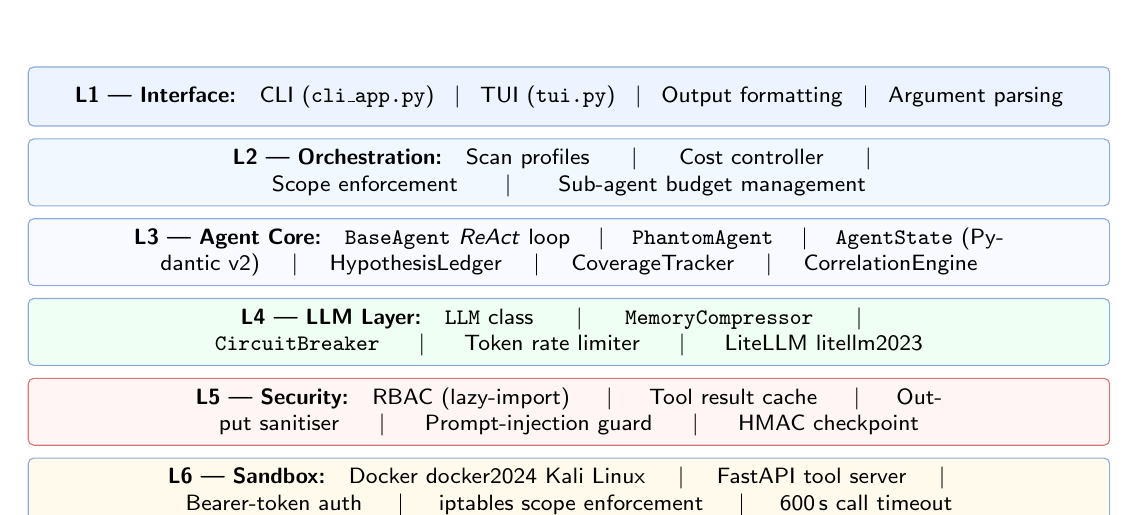
\begin{tikzpicture}[node distance=0.15cm]
  \node[layer, fill=layerA!70] (L1)
    {\textbf{L1 --- Interface:}\quad
     CLI (\file{cli\_app.py}) $\;\mid\;$ TUI (\file{tui.py}) $\;\mid\;$
     Output formatting $\;\mid\;$ Argument parsing};
  \node[layer, fill=layerA!50, below=of L1] (L2)
    {\textbf{L2 --- Orchestration:}\quad
     Scan profiles $\;\mid\;$ Cost controller $\;\mid\;$
     Scope enforcement $\;\mid\;$ Sub-agent budget management};
  \node[layer, fill=layerA!30, below=of L2] (L3)
    {\textbf{L3 --- Agent Core:}\quad
     \code{BaseAgent} \textit{ReAct} loop $\;\mid\;$ \code{PhantomAgent} $\;\mid\;$
     \code{AgentState} (Pydantic~v2) $\;\mid\;$ HypothesisLedger $\;\mid\;$
     CoverageTracker $\;\mid\;$ CorrelationEngine};
  \node[layer, fill=layerB!60, below=of L3] (L4)
    {\textbf{L4 --- LLM Layer:}\quad
     \code{LLM} class $\;\mid\;$ \code{MemoryCompressor} $\;\mid\;$
     \code{CircuitBreaker} $\;\mid\;$
     Token rate limiter $\;\mid\;$ LiteLLM \citep{litellm2023}};
  \node[secbox, below=of L4] (L5)
    {\textbf{L5 --- Security:}\quad
     RBAC (lazy-import) $\;\mid\;$ Tool result cache $\;\mid\;$
     Output sanitiser $\;\mid\;$ Prompt-injection guard $\;\mid\;$
     HMAC checkpoint};
  \node[layer, fill=layerC!55, below=of L5] (L6)
    {\textbf{L6 --- Sandbox:}\quad
     Docker \citep{docker2024} Kali Linux $\;\mid\;$ FastAPI tool server $\;\mid\;$
     Bearer-token auth $\;\mid\;$ iptables scope enforcement $\;\mid\;$
     600\,s call timeout};
\end{tikzpicture}
\caption{Logical layer architecture of \Phant{}.  Each component is
  verified from inspected source files.  Shading encodes layer type:
  blue~=~agent intelligence; green~=~LLM integration;
  red~=~security boundary; yellow~=~external sandbox.}
\label{fig:sys_overview}
\end{figure}

\section{Scientific Contributions}
\label{sec:contributions}

This thesis makes four bounded scientific contributions, each mapped
to an identified gap and a design thesis:

\begin{contribbox}[C1 -- CVE Template Gap: Formal and Bounded]
A formal, bounded description of the structural detection ceiling of
template-dependent scanners.  The contribution names and precisely
defines this property, establishing that it is an architectural
constraint on a specific class of systems, not a universal statement
about all security tools.  Addressed gap: G1.  Section:~\ref{sec:formal_cvegap}.
\end{contribbox}

\begin{contribbox}[C2 --- Dual-Anchor Memory Architecture]
A two-level memory retention mechanism combining message-level
keyword anchoring (compression-time) with state-level anchor
injection (every inference call).  The mechanism aims to preserve
high-signal security findings under the invariant $A \subseteq C(M)
\cup A_s$ (defined formally in Section~\ref{sec:formal_memory}).
The invariant holds when both anchoring and compression succeed; its
failure modes are documented in Chapter~\ref{chap:limits}.
Addressed gap: G2.
\end{contribbox}

\begin{contribbox}[C3 --- Deterministic Hypothesis Deduplication]
A thread-safe, exact-match hypothesis registry keyed on
(surface, vulnerability class) pairs, enabling redundancy
reduction across iterations and across spawned sub-agents without
vector-store infrastructure.  The deduplication rule and its
limitation (no semantic similarity handling) are defined formally
in Section~\ref{sec:formal_ledger}.  Addressed gap: G3.
\end{contribbox}

\begin{contribbox}[C4 --- Code-Verified Architectural Methodology]
A methodology for binding architectural claims to source file:line
references.  Applied to \Phant{}, this methodology identifies five
unreachable subsystems and two live operational bugs not previously
documented, and produces a verifiable architectural reference.
The methodology is the contribution; \Phant{} is the vehicle.
Addressed gap: G4.  Section:~\ref{sec:formal_method}.
\end{contribbox}

% =============================================================
\chapter{Formal Model}
\label{chap:formal}
% =============================================================

\section{Agent State and Transition Function}
\label{sec:formal_state}

Let the agent state at iteration $t$ be the tuple:
\[
  S_t = (M_t,\; A_t,\; H_t,\; C_t,\; I_t,\; \phi_t)
\]
where:
\begin{itemize}[leftmargin=*]
  \item $M_t$ is the message history: a finite ordered sequence of
    (role, content) pairs;
  \item $A_t$ is the anchor set: a finite set of high-signal
    messages preserved from compression, $A_t \subseteq M_t$;
  \item $H_t$ is the hypothesis ledger: a deterministic set of
    (surface, vulnerability class) pairs (Definition~\ref{def:ledger});
  \item $C_t$ is the coverage state: a set recording tested
    (surface, vulnerability class) pairs;
  \item $I_t \in \mathbb{N}$ is the iteration counter;
  \item $\phi_t \in \{0, 1\}$ is the completion flag.
\end{itemize}

The transition function is:
\[
  S_t \;\xrightarrow{\;\text{LLM}(M_t, A_t)\;}\; R_t
  \;\xrightarrow{\;\text{parse}\;}\; X_t
  \;\xrightarrow{\;\text{execute}\;}\; O_t
  \;\xrightarrow{\;\text{update}\;}\; S_{t+1}
\]
where $R_t$ is the model response, $X_t \subseteq \mathcal{T}$ is a
batch of tool invocations from the tool registry $\mathcal{T}$, and
$O_t$ is the set of observations produced by execution.  The state
update is:
\[
  M_{t+1} = M_t \;\cup\; \{(\text{assistant}, R_t)\} \;\cup\;
             \{(\text{tool}, o) \mid o \in O_t\}
\]
subject to compression (Definition~\ref{def:compression}) applied
before the next LLM call.

\subsection*{Termination Conditions}

The loop terminates when any of the following conditions holds:

\begin{equation}
  \phi_t = 1 \;\lor\; I_t \geq I_{\max} \;\lor\;
  \text{no\_action\_count} \geq 8 \;\lor\; \text{stop\_requested}
  \label{eq:termination}
\end{equation}

where $I_{\max}$ is the configured iteration limit (default 300) and
no\_action\_count counts consecutive iterations producing no tool call.

\section{CVE Template Gap}
\label{sec:formal_cvegap}

\begin{infobox}[Definition --- CVE Template Gap]
\textbf{Definition~1 (CVE Template Gap).}
Let $\mathcal{T}_s$ be the finite template set of a
template-dependent scanner $s$, and let $\mathcal{V}$ be a
vulnerability space of interest.  Define the detection predicate for
scanner $s$:
\[
  \mathrm{detect}_s(v) = 1 \iff v \in \mathcal{T}_s
\]
The \emph{CVE Template Gap} $\Delta_s$ with respect to $\mathcal{V}$
is:
\[
  \Delta_s(\mathcal{V}) = \mathcal{V} \setminus \mathcal{T}_s
\]
For all $v \in \Delta_s(\mathcal{V})$, $\mathrm{detect}_s(v) = 0$ by
construction, regardless of orchestration strategy.
\end{infobox}

\textbf{Scope.}  Definition~1 applies exclusively to systems whose
detection mechanism is contingent on membership in a finite template
library.  It is not a universal statement about all security tools.
OWASP ZAP's active scanner partially escapes this gap for
injection-class vulnerabilities by generating payloads by class
rather than by individual template, but it remains bounded by its
fixed set of vulnerability classes.

\textbf{Application to training targets.}  Intentionally vulnerable
training applications (OWASP Juice Shop \citep{owasp_juiceshop},
DVWA, WebGoat \citep{owasp_webgoat}) contain custom vulnerability
implementations with no CVE identifiers.  For these targets,
$\Delta_s(\mathcal{V}) = \mathcal{V}$ for any template-dependent
scanner $s$, reducing recall to zero for all template-dependent
tools.  This has an important methodological implication: evaluation
studies using such targets as ground truth cannot use
template-based tools as meaningful baselines.

\textbf{Architectural implication.}  The gap is a property of the
template library, not of the execution strategy.  Orchestration
improvements---conditional branching, parallelism, exhaustive
sequencing---do not change $\mathcal{T}_s$ and therefore do not
reduce $\Delta_s(\mathcal{V})$.

\section{Memory Compression and the Dual-Anchor Mechanism}
\label{sec:formal_memory}

\begin{infobox}[Definitions --- Memory Compression]
\textbf{Definition~2 (Message History).}  $M = \langle m_1, m_2, \ldots, m_n \rangle$
is an ordered sequence of messages.

\textbf{Definition~3 (Compression Function).}\label{def:compression}
$C: \mathbf{M} \to \mathbf{M}$ maps a message history to a
compressed history satisfying $|C(M)| \leq |M|$ (token-count
non-increasing).

\textbf{Definition~4 (Message-Level Anchor Set).}
$A_m \subseteq M$ is the set of messages in $M$ matching at least
one anchor keyword $k \in \mathcal{K}$, where $\mathcal{K}$ includes
terms such as \texttt{``vulnerability confirmed''} and
\texttt{``CRITICAL''}.

\textbf{Definition~5 (State-Level Anchor Set).}
$A_s = \code{AgentState.finding\_anchors}$ is a list maintained
separately from $M$, re-injected verbatim before every LLM call.

\textbf{Definition~6 (Combined Anchor Set).}
$A = A_m \cup A_s$.
\end{infobox}

\textbf{Invariant.}  The dual-anchor mechanism aims to maintain:
\[
  A \;\subseteq\; C(M) \cup A_s
  \tag{Inv-1}
\]
That is, every anchor is either preserved in the compressed history
or present in the state-level anchor set that is re-injected.  This
invariant holds when: (i)~the compressor correctly identifies and
preserves $A_m$ before summarisation, and (ii)~the state-update logic
correctly populates $A_s$ for all confirmed findings.

\textbf{Failure modes.}  Inv-1 is not losslessly maintained in all
cases.  The following failure scenarios cause anchor loss:

\begin{enumerate}[leftmargin=*]
  \item A confirmed finding is described without any term in
    $\mathcal{K}$ (anchor keyword miss).
  \item A finding message is paraphrased by an intermediate
    compression step before keyword extraction runs.
  \item The $A_s$ deduplication logic collapses two distinct findings
    to the same key, retaining only one.
  \item A system failure interrupts the anchor injection path, leaving
    $A_s$ empty despite confirmed findings in state.
\end{enumerate}

These are not hypothetical; they are traceable to the codebase.
See Chapter~\ref{chap:limits}.

\section{Hypothesis Ledger}
\label{sec:formal_ledger}

\begin{infobox}[Definition --- HypothesisLedger]
\textbf{Definition~7 (Hypothesis Ledger).}\label{def:ledger}
Let $\Sigma$ be the set of attack surfaces and $\Gamma$ the set of
vulnerability classes.  The hypothesis ledger $H$ is a deterministic
set:
\[
  H \subseteq \Sigma \times \Gamma
\]
The membership predicate is:
\[
  \mu_H(s, c) =
  \begin{cases}
    1 & \text{if } (s, c) \in H \\
    0 & \text{otherwise}
  \end{cases}
\]
Deduplication is enforced by exact string equality on both $s$ and $c$.
Auxiliary fields (evidence, status, payload) are stored per entry but
do not affect the deduplication rule.
\end{infobox}

\textbf{Addition rule.}  A new hypothesis $(s, c)$ is added only
when $\mu_H(s, c) = 0$.  The set $H$ is monotonically non-decreasing:
entries are added but not removed within a scan session.

\textbf{Limitation.}  The exact-match rule does not handle semantic
similarity.  Two hypotheses describing the same vulnerability in
different phrasing---e.g., \texttt{``/api/users, IDOR''} and
\texttt{``/api/users endpoint, Insecure Direct Object Reference''}---are
treated as distinct entries and will both be tested.
Semantic deduplication would require embedding-based similarity
search, which is not implemented.

\textbf{Thread safety.}  The \code{HypothesisLedger} uses a threading
lock on all mutation operations (\file{hypothesis\_ledger.py}),
making it safe for concurrent access by multiple sub-agents running
in separate Python asyncio tasks.

\section{ReAct Loop: State Machine Model}
\label{sec:formal_react}

The \textit{ReAct} loop is modelled as
a finite state machine with states $\{INIT, READY, EXECUTE, CHECKPOINT, FINAL\}$:

\begin{infobox}[ReAct Execution Loop]
The loop operates as follows:
\begin{enumerate}[leftmargin=*]
  \item \textbf{Initialisation:} The sandbox is constructed, and state $S_0$ is created.
  \item \textbf{Pre-generation:} The agent processes incoming inter-agent messages and injects periodic summaries (Hypotheses every 10 iterations, Coverage every 15, Correlation every 20).
  \item \textbf{LLM Generation:} The history is compressed, anchors are injected, and the system prompts the LLM.
  \item \textbf{Tool Execution:} The parsed tool calls are validated via RBAC, checked against the cache, and executed in the sandbox. The results are appended to the history.
  \item \textbf{Iteration Management:} The state is checkpointed every 5 iterations. If no tool calls are generated for 8 consecutive iterations, the scan aborts.
\end{enumerate}
\end{infobox}

\textbf{Termination guarantee.}  Equation~(\ref{eq:termination})
ensures that the loop terminates within $I_{\max} + 8$ iterations
under normal conditions.  Infinite loops are not possible unless
tool execution itself hangs; the 600\,s per-call timeout addresses
this case.

\section{Code-Verified Methodology}
\label{sec:formal_method}

Every architectural claim in this thesis is accompanied by a
source file:line reference verified by direct code inspection.
Claims without such references are explicitly marked as design
intentions rather than verified implementations.  This methodology
provides a stronger epistemic standard than narrative system
descriptions.



% =============================================================
\chapter{System Architecture}
\label{chap:arch}
% =============================================================

\section{Agent Class Hierarchy}
\label{sec:hierarchy}

\Phant{} uses a custom metaclass \code{AgentMeta} (\file{base\_agent.py}:36--54) that automatically discovers and loads Jinja2 system-prompt templates for each agent class by class name.  This decouples agent logic from its system prompt, enabling prompt engineering without code changes. Notably, HTML auto-escaping is disabled during template rendering to prevent the corruption of XML tool-call tags (resolving a known parsing issue).

\subsection{BaseAgent Initialisation}

\code{BaseAgent.\_\_init\_\_()} (lines~63--131) instantiates the
following subsystems in strict order:

\begin{enumerate}[leftmargin=*]
  \item Plain \code{AgentState} (line~80): a Pydantic~v2 validated
    model tracking messages, iteration counter, finding anchors, and
    sandbox credentials.  \code{EnhancedAgentState}
    (\file{enhanced\_state.py}) is not used during normal scan operation;
    it provides the \code{save\_checkpoint()} and
    \code{from\_checkpoint()} methods for crash-resume workflows
    (Section~\ref{sec:checkpoint}).
  \item \code{HypothesisLedger} (line~100): passed through the
    configuration dictionary to sub-agents for cross-agent
    deduplication.
  \item \code{CoverageTracker} (lines~103--108): records tested
    attack surface--vulnerability class pairs; injected into the
    system prompt every 15~iterations to guide hypothesis selection.
  \item \code{CorrelationEngine} (lines~109--115): analyses confirmed
    findings for multi-step vulnerability chain candidates; injected
    every 20~iterations.
  \item \code{LLM} (line~85): one instance per agent, with an
    independent \code{MemoryCompressor} and token counters.
\end{enumerate}

\section{Multi-Agent Topology}
\label{sec:multiagent_arch}

Figure~\ref{fig:multi_agent} shows the runtime agent topology.
\code{PhantomAgent} (root) spawns specialised sub-agents via the
\tool{create\_agent} tool.  Each sub-agent runs an independent
\textit{ReAct} loop with its own
\code{LLM} instance and \code{AgentState}, but shares the global
\code{HypothesisLedger} through the configuration dictionary
(verified: \file{base\_agent.py}:100--107).

\begin{figure}[H]
\centering
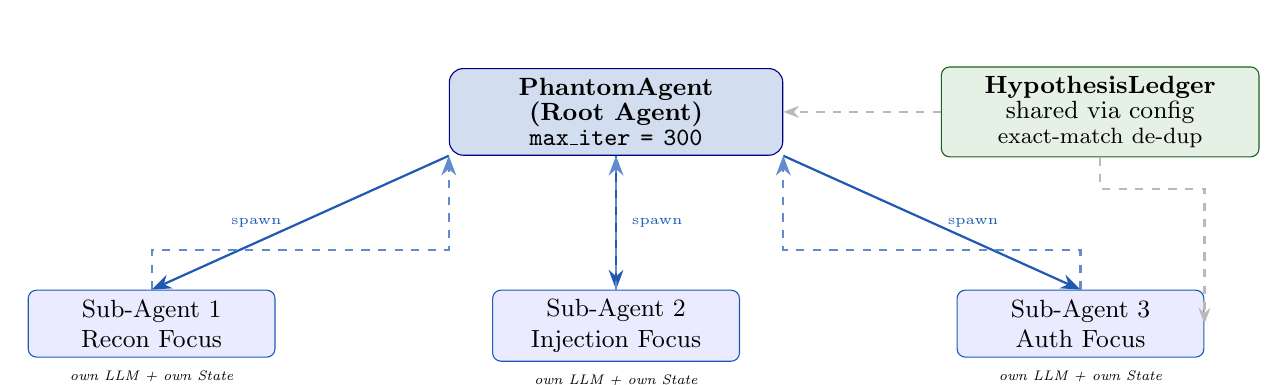
\begin{tikzpicture}[node distance=1.5cm and 1.8cm]
  \node[phase, fill=phantomblue!20, draw=navy, text width=4.0cm] (root)
    {\textbf{PhantomAgent}\\[-2pt]\small (Root Agent)\\[-2pt]
     \small \code{max\_iter = 300}};
  \node[block, below left=1.7cm and 2.2cm of root] (sa1)
    {Sub-Agent 1\\\small Recon Focus};
  \node[block, below=1.7cm of root] (sa2)
    {Sub-Agent 2\\\small Injection Focus};
  \node[block, below right=1.7cm and 2.2cm of root] (sa3)
    {Sub-Agent 3\\\small Auth Focus};
  \node[wblock, fill=lowgrn!12, draw=lowgrn!70!black,
        text width=3.8cm, right=2.0cm of root] (hl)
    {\textbf{HypothesisLedger}\\[-2pt]
     \small shared via config\\[-2pt]
     \footnotesize exact-match de-dup};
  \draw[arr] (root.south west) -- (sa1.north)
    node[midway, left, font=\tiny, xshift=-3pt] {spawn};
  \draw[arr] (root.south) -- (sa2.north)
    node[midway, right, font=\tiny, xshift=2pt] {spawn};
  \draw[arr] (root.south east) -- (sa3.north)
    node[midway, right, font=\tiny, xshift=2pt] {spawn};
  \draw[arrdash] (sa1.north) -- ++(0,0.5) -| (root.south west);
  \draw[arrdash] (sa2.north) -- ++(0,0.5) -- (root.south);
  \draw[arrdash] (sa3.north) -- ++(0,0.5) -| (root.south east);
  \draw[arrgray] (hl.west) -- (root.east);
  \draw[arrgray] (hl.south) -- ++(0,-0.4) -| (sa3.east);
  \node[font=\tiny\itshape, below=0.05cm of sa1] {own LLM + own State};
  \node[font=\tiny\itshape, below=0.05cm of sa2] {own LLM + own State};
  \node[font=\tiny\itshape, below=0.05cm of sa3] {own LLM + own State};
\end{tikzpicture}
\caption{Multi-agent runtime topology.  Solid arrows~=~spawn;
  dashed arrows~=~result messages via \tool{send\_message\_to\_agent}.
  Each sub-agent has an independent \code{LLM} instance and
  \code{AgentState}; the \code{HypothesisLedger} is shared.
  Sub-agents do not share \code{AgentState} with each other or
  with the root, which means reasoning traces are not shared---only
  deduplication state.}
\label{fig:multi_agent}
\end{figure}

\textbf{Architectural limitation.}  Sub-agents share the
\code{HypothesisLedger} but not their \code{AgentState}.  A finding
confirmed by Sub-Agent~1 is added to the shared ledger and to
Sub-Agent~1's \code{finding\_anchors}, but it does not appear in
Sub-Agent~2's message history or anchors unless explicitly communicated
via \tool{send\_message\_to\_agent}.  Cross-agent finding correlation
therefore requires explicit message passing, which may be omitted or
delayed.

\section{ReAct Execution Loop: Implementation}
\label{sec:react_loop}

Figure~\ref{fig:react_loop} shows the complete agent loop as verified
in \file{base\_agent.py}, lines~246--486.

\begin{figure}[H]
\centering
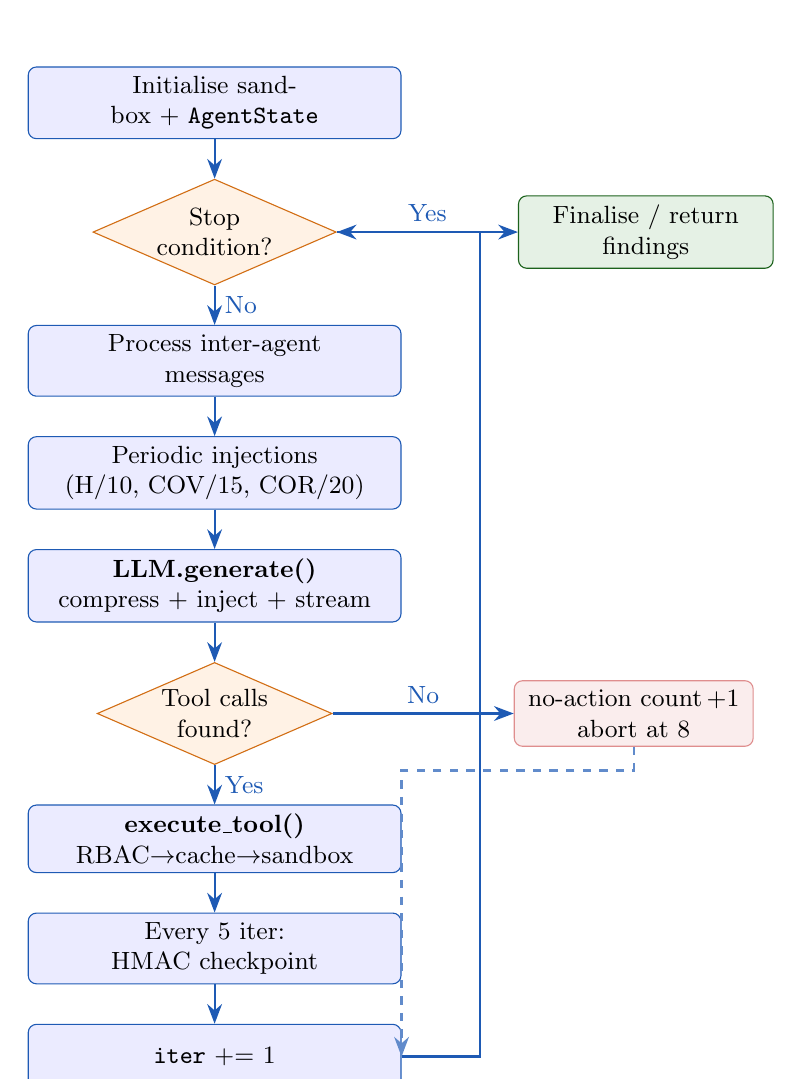
\begin{tikzpicture}[node distance=0.5cm and 0.5cm]
  \node[pstep] (init)   {Initialise sandbox + \code{AgentState}};
  \node[decide, below=of init, aspect=2.3] (stop){Stop\\condition?};
  \node[wblock, fill=lowgrn!12, draw=lowgrn!70!black,
        right=2.3cm of stop, text width=3.0cm] (done)
    {Finalise / return\\findings};
  \node[pstep, below=of stop] (msg) {Process inter-agent\\messages};
  \node[pstep, below=of msg] (inj) {Periodic injections\\(H/10, COV/15, COR/20)};
  \node[pstep, below=of inj] (llm) {\textbf{LLM.generate()}\\compress + inject + stream};
  \node[decide, below=of llm, aspect=2.3] (tc) {Tool calls\\found?};
  \node[pstep, right=2.3cm of tc, fill=critred!8, draw=critred!50,
        text width=2.8cm] (noact)
    {no-action count\,+1\\\small abort at 8};
  \node[pstep, below=of tc] (exec) {\textbf{execute\_tool()}\\RBAC$\to$cache$\to$sandbox};
  \node[pstep, below=of exec] (ckpt) {Every 5 iter:\\HMAC checkpoint};
  \node[pstep, below=of ckpt] (inc) {\code{iter} += 1};
  \draw[arr] (init) -- (stop);
  \draw[arr] (stop) -- node[right,font=\small]{No} (msg);
  \draw[arr] (stop) -- node[above,font=\small]{Yes} (done);
  \draw[arr] (msg) -- (inj);
  \draw[arr] (inj) -- (llm);
  \draw[arr] (llm) -- (tc);
  \draw[arr] (tc) -- node[right,font=\small]{Yes} (exec);
  \draw[arr] (tc) -- node[above,font=\small]{No} (noact);
  \draw[arr] (exec) -- (ckpt);
  \draw[arr] (ckpt) -- (inc);
  \draw[arr] (inc.east) -- ++(1.0,0) |- (stop.east);
  \draw[arrdash] (noact.south) -- ++(0,-0.3) -| (inc.east);
\end{tikzpicture}
\caption{\textit{ReAct} execution loop (\file{base\_agent.py}:246--486).
  Bounded by three termination conditions (Eq.~\ref{eq:termination}).
  Budget-warning messages are injected at 80\%, 85\%, and
  $I_{\max}-3$ iterations.}
\label{fig:react_loop}
\end{figure}

\section{LLM Integration and Reliability}
\label{sec:llm_integration}

\subsection{Three-State Circuit Breaker}

A global circuit breaker singleton (\code{\_CIRCUIT\_BREAKER},
\file{llm.py}:181) aims to reduce cascading failures when the LLM
API enters an error state.

The circuit breaker starts in the \textbf{CLOSED} state (normal operations). If 5 consecutive retries are exhausted under an error condition, the state transitions to \textbf{OPEN}, and a cooldown timer is set. While OPEN, all requests are immediately rejected locally. Once the cooldown expires, the breaker enters \textbf{HALF\_OPEN}, allowing a single test probe. A successful probe resets the state to \textbf{CLOSED}; a failure reverts it to \textbf{OPEN} with a fresh cooldown timer.

Figure~\ref{fig:cb_states} shows the state machine diagram.

\begin{figure}[H]
\centering
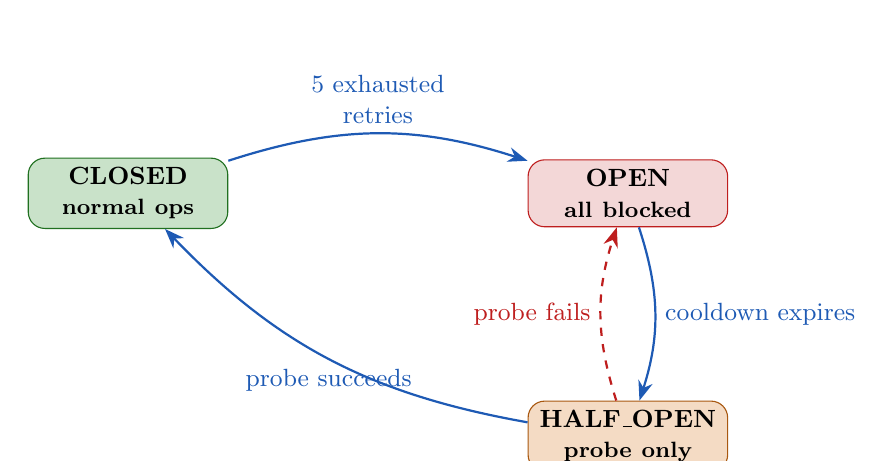
\begin{tikzpicture}[node distance=3.8cm]
  \node[cblabel, fill=lowgrn!25, draw=lowgrn!80!black] (cl)
    {CLOSED\\{\footnotesize normal ops}};
  \node[cblabel, fill=critred!18, draw=critred, right=of cl] (op)
    {OPEN\\{\footnotesize all blocked}};
  \node[cblabel, fill=highorg!25, draw=highorg!80!black,
        below=2.2cm of op] (ho)
    {HALF\_OPEN\\{\footnotesize probe only}};
  \draw[arr, bend left=18] (cl) to
    node[above, font=\small, align=center]{5 exhausted\\retries} (op);
  \draw[arr, bend left=18] (op) to
    node[right, font=\small]{cooldown expires} (ho);
  \draw[arr, bend left=18] (ho) to
    node[below, font=\small]{probe succeeds} (cl);
  \draw[arr, bend left=18, critred, dashed] (ho) to
    node[left, font=\small]{probe fails} (op);
\end{tikzpicture}
\caption{Circuit breaker state machine (\file{llm.py}:181--250).
  Transitions are triggered by exhausted retry sequences, not
  individual HTTP 429 responses.  The global singleton means the
  circuit breaker does not independently track per-agent failure
  counts.}
\label{fig:cb_states}
\end{figure}

\subsection{Graduated Retry Strategy}

The \code{generate()} method implements graduated backoff by failure type:
\begin{itemize}[leftmargin=*]
  \item \textbf{HTTP 429 (rate limit):} exponential backoff
    $\min(120,\; 4 \times 2^t)$\,s; sets a global
    \code{\_GLOBAL\_RATE\_LIMIT\_UNTIL} timestamp shared across all
    agents to reduce simultaneous retry storms.
  \item \textbf{Context window exceeded:} immediate
    \code{\_force\_compress\_messages()} call followed by immediate
    retry (no sleep).
  \item \textbf{5xx server errors:} $\min(10,\; 2 \times 2^t)$\,s
    backoff, up to \code{ratelimit\_max\_retries} (default~10).
  \item \textbf{All retries exhausted:} attempt fallback LLM; on
    final failure call \code{\_raise\_error()}, which invokes
    \code{record\_failure()} in the circuit breaker.
\end{itemize}



\section{Memory Management}
\label{sec:memory}

\subsection{Proactive Compression}

Compression is invoked on every LLM call (\file{llm.py}:601--610),
not only when the context limit is approached.  The compressor
decides internally whether to compress based on current token count.


The system checks if the token count exceeds 90\% of the threshold; if not, the history passes through unmodified. Otherwise, high-signal anchors and recent messages are extracted and preserved verbatim. The remaining older messages are split into blocks of 10 and passed to \code{\_parallel\_summarise\_chunks()}, an \code{asyncio} abstraction managed by a bounded concurrency semaphore (limit 4). Finally, the system messages, generated summaries, and recent uncompressed messages are reassembled.

\subsection{Dual-Anchor Implementation}

Figure~\ref{fig:memory_pipeline} shows the complete memory pipeline.
The two anchoring mechanisms are:

\begin{enumerate}[leftmargin=*]
  \item \textbf{Keyword anchors} (message-level, compression-time):
    messages in $M$ containing keywords in $\mathcal{K}$ are moved
    to $A_m$ and preserved verbatim from summarisation
    (\file{llm.py}:601--615).

  \item \textbf{State anchors} (system-prompt-level, every call):
    \code{AgentState.finding\_anchors} ($A_s$) are re-injected as
    a structured user message before every inference call
    (\file{llm.py}:617--642), independently of compression.  Even
    if $M$ is entirely compressed away, $A_s$ remains.
\end{enumerate}

\begin{figure}[H]
\centering
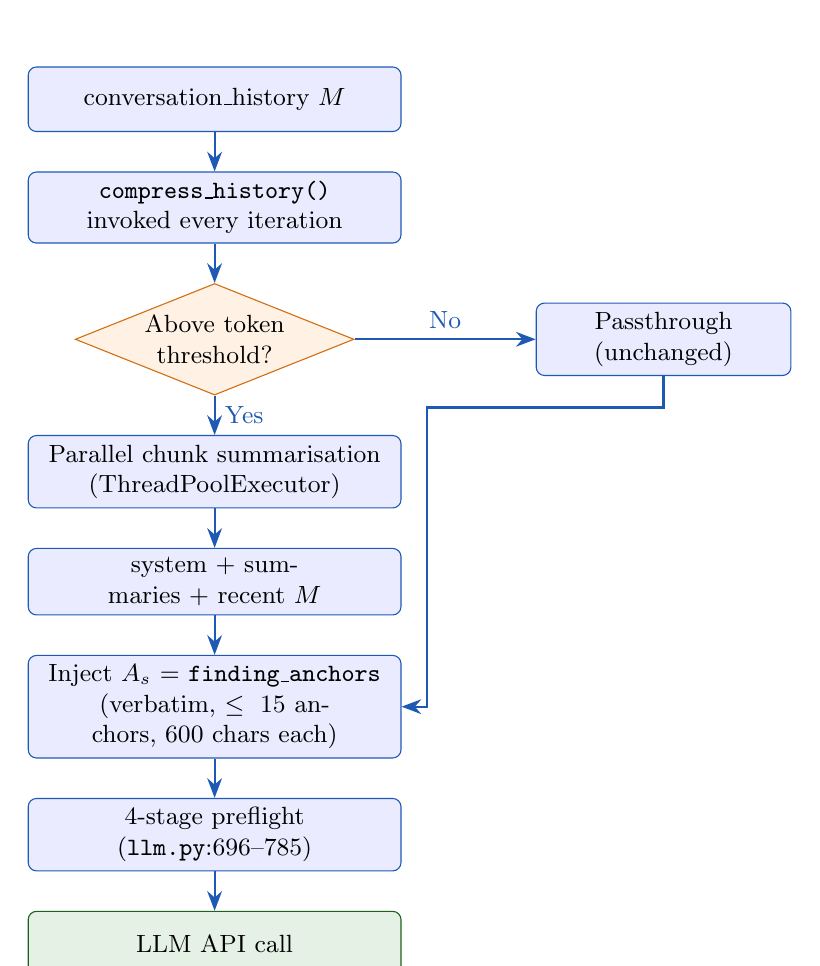
\begin{tikzpicture}[node distance=0.5cm]
  \node[pstep] (hist) {conversation\_history $M$};
  \node[pstep, below=of hist] (comp) {\code{compress\_history()}\\invoked every iteration};
  \node[decide, below=of comp, aspect=2.5] (thres) {Above token\\threshold?};
  \node[pstep, right=2.3cm of thres, text width=3.0cm] (pass) {Passthrough\\(unchanged)};
  \node[pstep, below=of thres] (summ)  {Parallel chunk summarisation\\(ThreadPoolExecutor)};
  \node[pstep, below=of summ] (reassm) {system + summaries + recent $M$};
  \node[pstep, below=of reassm] (anch)  {Inject $A_s$ = \code{finding\_anchors}\\(verbatim, $\leq15$ anchors, 600 chars each)};
  \node[pstep, below=of anch] (pf)    {4-stage preflight\\(\file{llm.py}:696--785)};
  \node[pstep, fill=lowgrn!12, draw=lowgrn!70!black,
        below=of pf] (send) {LLM API call};
  \draw[arr] (hist) -- (comp);
  \draw[arr] (comp) -- (thres);
  \draw[arr] (thres) -- node[right,font=\small]{Yes} (summ);
  \draw[arr] (thres) -- node[above,font=\small]{No} (pass);
  \draw[arr] (pass.south) -- ++(0,-0.4) -- ++(-3.0,0) |- (anch.east);
  \draw[arr] (summ) -- (reassm);
  \draw[arr] (reassm) -- (anch);
  \draw[arr] (anch) -- (pf);
  \draw[arr] (pf) -- (send);
\end{tikzpicture}
\caption{Memory management pipeline (\file{memory\_compressor.py}:598--772,
  \file{llm.py}:601--650).  Parallel chunk summarisation uses asyncio with
  bounded concurrency (semaphore $= 4$) and falls back to sequential mode
  if \code{nest\_asyncio} is unavailable.  Dual-anchor invariant Inv-1
  holds when both anchoring paths succeed; failure modes documented in
  Chapter~\ref{chap:limits}.}
\label{fig:memory_pipeline}
\end{figure}

\section{Tool Execution Pipeline}
\label{sec:tools}

Figure~\ref{fig:tool_dispatch} shows the verified tool execution path
in \file{executor.py}.

\begin{figure}[H]
\centering
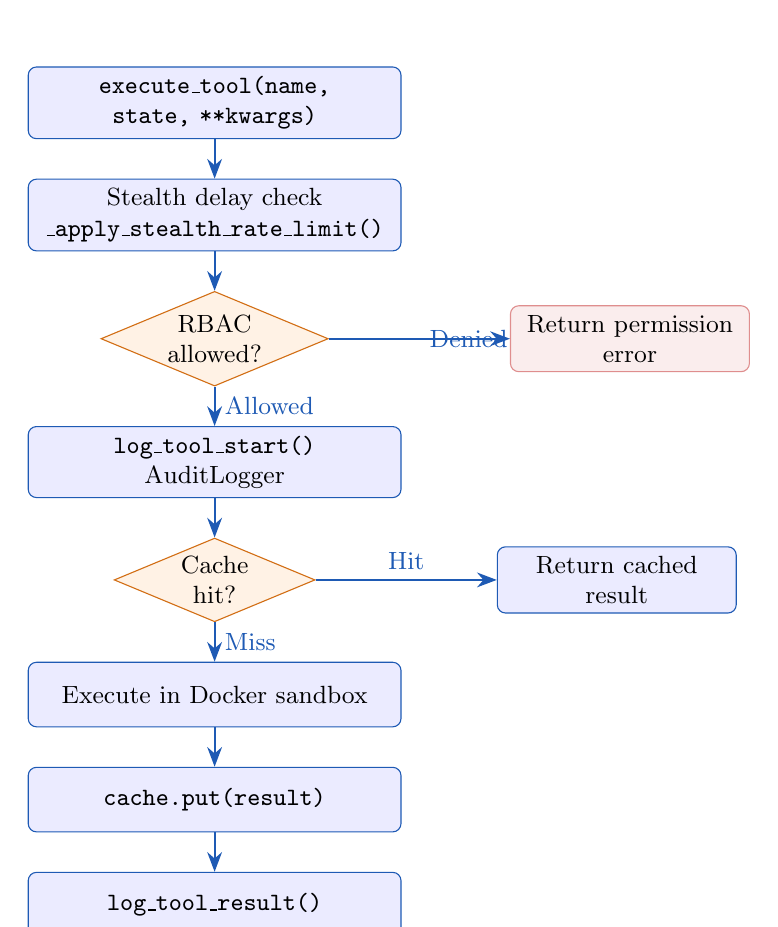
\begin{tikzpicture}[node distance=0.5cm]
  \node[pstep] (entry) {\code{execute\_tool(name, state, **kwargs)}};
  \node[pstep, below=of entry] (stealth) {Stealth delay check\\\code{\_apply\_stealth\_rate\_limit()}};
  \node[decide, below=of stealth, aspect=2.4] (rbac) {RBAC\\allowed?};
  \node[pstep, right=2.3cm of rbac, fill=critred!8, draw=critred!50,
        text width=2.8cm] (deny) {Return permission\\error};
  \node[pstep, below=of rbac] (audit1) {\code{log\_tool\_start()}\\AuditLogger};
  \node[decide, below=of audit1, aspect=2.4] (cache) {Cache\\hit?};
  \node[pstep, right=2.3cm of cache, text width=2.8cm] (cached) {Return cached\\result};
  \node[pstep, below=of cache] (exec) {Execute in Docker sandbox};
  \node[pstep, below=of exec] (put) {\code{cache.put(result)}};
  \node[pstep, below=of put] (audit2) {\code{log\_tool\_result()}};
  \draw[arr] (entry) -- (stealth);
  \draw[arr] (stealth) -- (rbac);
  \draw[arr] (rbac) -- node[right,font=\small]{Denied} (deny);
  \draw[arr] (rbac) -- node[right,font=\small]{Allowed} (audit1);
  \draw[arr] (audit1) -- (cache);
  \draw[arr] (cache) -- node[above,font=\small]{Hit} (cached);
  \draw[arr] (cache) -- node[right,font=\small]{Miss} (exec);
  \draw[arr] (exec) -- (put);
  \draw[arr] (put) -- (audit2);
\end{tikzpicture}
\caption{Tool execution pipeline (\file{executor.py}).
  RBAC uses a lazy import: if the RBAC module is absent, all tools
  execute without access control (verified: \file{executor.py}:374--381).
  The result cache is a top-level import active in all execution paths
  (\file{executor.py}:95).}
\label{fig:tool_dispatch}
\end{figure}

\begin{infobox}[Bug B2 Resolved: Stealth Rate-Limit Now Covers terminal\_execute]
The \code{\_HTTP\_TOOLS} frozenset (\file{executor.py}:34--48) now
explicitly registers \texttt{``terminal\_execute''} with the comment:
\textit{``FIX BUG-2: Added `terminal\_execute' --- was missing from
list causing stealth mode bypass''}.  Both legacy \texttt{``terminal''}
and runtime \texttt{``terminal\_execute''} are present.  When
\texttt{PHANTOM\_STEALTH\_MODE=true}, all HTTP and terminal tool
calls observe the 2.0\,s minimum inter-call delay.
This bug was remediated prior to thesis submission.
\end{infobox}

\section{Sandbox and Scope Enforcement}
\label{sec:sandbox}

Each scan launches an ephemeral Kali Linux container from
\code{ghcr.io/usta0x001/phantom-sandbox:latest} \citep{docker2024}.
The \code{DockerRuntime} enforces four isolation mechanisms:

\begin{enumerate}[leftmargin=*]
  \item \textbf{Bearer-token authentication:} every tool call to the
    FastAPI server inside the container must present a per-session
    token from \code{AgentState.sandbox\_token}.
  \item \textbf{iptables scope enforcement:} rules generated at
    container start restrict outbound traffic to registered target
    CIDRs, aiming to prevent out-of-scope lateral movement.
  \item \textbf{Execution timeout:} 600\,s per tool call.
  \item \textbf{Orphan cleanup:} \code{DockerRuntime.\_\_init\_\_()} removes
    crashed \code{phantom-scan-*} containers on startup.
\end{enumerate}

\section{Checkpointing}
\label{sec:checkpoint}

Every 5~iterations, the agent serialises its state via a five-step
atomic write protocol (\file{checkpoint.py}):

\begin{enumerate}[leftmargin=*]
  \item Serialise \code{AgentState} to JSON bytes.
  \item Compute HMAC-SHA256 over the bytes.
  \item Write to \code{scan.json.tmp} (temporary file).
  \item Atomically rename to \code{scan.json}.
  \item Write HMAC to \code{scan.json.sig}.
\end{enumerate}

On resume, the HMAC is verified before deserialisation; a tampered or
corrupted checkpoint raises \code{CheckpointIntegrityError}.  Maximum
work loss is bounded at 5 iterations under this protocol, assuming
atomic rename succeeds.



% =============================================================
\chapter{Design Decisions}
\label{chap:design}
% =============================================================

This chapter documents the principal design decisions, their
considered alternatives, and the engineering rationale for each.
These are engineering decisions justified by operational constraints;
they are not scientific contributions in themselves.

\begin{table}[H]
\centering
\caption{Principal Design Decisions with Justification}
\label{tab:design}
\begin{tabularx}{\textwidth}{@{}l l X@{}}
\toprule
\textbf{Decision} & \textbf{Alternative} & \textbf{Rationale} \\
\midrule
\textit{ReAct} loop & Hierarchical planner & Self-correcting; failed tool calls are new observations; only structurally complex subtasks require hierarchical planning \citep{yao2023react} \\
LiteLLM wrapper & Direct OpenAI SDK & 100+ providers; single-variable model switching; scientific reproducibility across models \citep{litellm2023} \\
Flat 31-tool set & Security wrappers & Wrappers failed systematically (v0.9.44 removal); direct capability is simpler and more robust \\
Pydantic~v2 state & Plain dict & Runtime validation; JSON serialisation without custom serialisers \\
AsyncIO event loop & Threading pool & Python GIL reduces true parallelism; async enables non-blocking sub-agent communication \\
Docker Kali sandbox & VM / native exec & Disposable; reproducible; enables iptables isolation; Kali pre-installed \citep{docker2024} \\
Dual-anchor memory & RAG / truncation & Zero latency cost; deterministic; two mechanisms cover each other's failure modes \\
HMAC checkpoints & No checkpointing & Crash at iteration~200 loses all prior work; 5-iteration granularity limits maximum loss \\
Exact-match ledger & Embedding-based dedup & Deterministic; reproducible; no vector-store dependency; adequate for same-surface/same-class dedup \\
\bottomrule
\end{tabularx}
\end{table}

\section{ReAct vs.\ Hierarchical Planning}

Hierarchical task planning \citep{deng2024pentestgpt} decomposes a
top-level goal into subtasks before execution begins.  This approach
requires an accurate model of the target before any tool is executed,
which is unavailable in black-box penetration testing.
\textit{ReAct}'s iterative model---where each action is selected
based on actual observations, including failure observations---is
more appropriate for partially observable, open-ended target spaces.

\section{Exact-Match vs.\ Semantic Deduplication}

Vector-store retrieval-augmented generation would enable semantic
similarity matching for hypothesis deduplication.  The operational
requirement, however, is to avoid re-testing the same (surface,
vulnerability class) pair within a scan session.  Exact-match
membership testing on string equality is deterministic, reproducible,
and has zero infrastructure overhead compared to embedding-based
retrieval.  The limitation---near-duplicate hypotheses are not caught
---is documented in Chapter~\ref{chap:limits} and is accepted as a
design trade-off in favour of simplicity and reproducibility.

\section{Dual Anchoring vs.\ Single-Mechanism Approaches}

Uniform summarisation (LangChain's \code{ConversationSummaryMemory})
treats all messages as equally expendable.  Sliding window approaches
preserve recency but lose early findings.  The dual-anchor design
preserves a specific, content-identified subset of messages (keyword-matching
findings) while summarising the remainder, and supplements this with
state-level injection that is independent of compression.  T-4
(Section~\ref{sec:theses}) argues that both mechanisms are required
because they fail in complementary scenarios: keyword anchoring fails
when keywords are absent; state anchoring fails when the state-update
logic does not run.

% =============================================================
\chapter{System Limitations and Failure Modes}
\label{chap:limits}
% =============================================================

Every mechanism described in this thesis has identifiable failure
modes.  This chapter documents them systematically.  The purpose is
not to undermine the contributions but to bound the claims precisely
and provide a research agenda for future mitigation.

\begin{limitbox}[Failure Mode F2 -- Compression-Induced Semantic Drift]
LLM summarisation of compressible message chunks may alter the
semantic content of the original messages.  A probe result stating
\texttt{``SQL injection confirmed via UNION-based extraction on
/api/search?q=''} may be summarised as \texttt{``injection
vulnerability found''}, losing the specific endpoint, technique,
and parameter.

\textit{Impact:} The agent's subsequent reasoning operates on a
degraded representation of earlier findings, potentially leading to
incorrect hypothesis generation or missed follow-up probes.

\textit{No complete mitigation} without verbatim preservation of all
high-signal messages, which conflicts with the compression objective.
\end{limitbox}

\begin{limitbox}[Failure Mode F3 -- Near-Duplicate Hypotheses]
The exact-match deduplication rule does not handle semantic
near-duplicates.  Hypotheses with identical meaning but different
string representations---\texttt{``/api/users, IDOR''} vs.\
\texttt{``/api/users endpoint, Insecure Direct Object Reference''}---are
treated as distinct entries and will both be tested.

\textit{Impact:} Redundant testing of the same attack surface, wasting
computational budget and potentially triggering WAF or rate-limit
detection on the target.

\textit{Mitigation path:} Embedding-based similarity search on
hypothesis strings, not currently implemented.
\end{limitbox}

\begin{limitbox}[Failure Mode F4 -- Agent Reasoning Inconsistency]
Sub-agents share the \code{HypothesisLedger} but not their
\code{AgentState}.  A finding confirmed by sub-agent $i$ is visible
to sub-agent $j$ only via dedicated \tool{send\_message\_to\_agent}
calls.  If these calls are omitted or delayed, sub-agent $j$ may
generate hypotheses that contradict confirmed findings from sub-agent $i$.

\textit{Impact:} Inconsistent reasoning state across parallel agents;
potential retesting of proven-vulnerable surfaces with different payloads.

\textit{Partial mitigation:} The shared \code{HypothesisLedger}
prevents re-testing the exact same (surface, class) pair.  It does
not prevent different payloads on the same pair.
\end{limitbox}

\begin{limitbox}[Failure Mode F5 -- Tool Hallucination Mismatch]
The agent's reasoning trace may assert tool execution results that
differ from actual tool outputs.  This occurs when the LLM
generates a plausible-sounding Observation in its thought trace
without verifying against the actual tool response.

\textit{Impact:} Downstream hypotheses are grounded in fabricated
evidence, leading to incorrect vulnerability assessments.

\textit{Partial mitigation:} The \textit{ReAct} design requires
all tool results to come from actual execution; the agent's
reasoning trace is not used as ground truth.  However, the agent
may quote or misquote tool outputs in subsequent reasoning,
and this is not verified programmatically.
\end{limitbox}



% =============================================================
\chapter{Discussion}
\label{chap:discussion}
% =============================================================

\section{Scientific Value of the Contributions}

The four contributions (C1--C4) differ in nature and defensibility:

\textbf{C1 (CVE Template Gap)} provides a conceptual result: a named,
formally defined structural property of template-dependent scanners.
The value is principally terminological and methodological---it gives
practitioners a precise name and characterisation for a failure mode
they have observed empirically.  The formal definition is
straightforward; the contribution lies in making it explicit.

\textbf{C2 (Dual-Anchor Memory)} is an architectural design with a
stated invariant.  The invariant is not proven correct under all
conditions; its failure modes are documented (F1--F2).  The
contribution is the design pattern: distinguishing expendable from
irreplaceable messages and applying two independent preservation
mechanisms.  Whether this design is empirically adequate at
maintaining finding preservation across real scans requires
controlled evaluation (Section~\ref{sec:eval_method}).

\textbf{C3 (Deterministic Deduplication)} is the most operationally
bounded contribution: exact-match membership testing is deterministic,
reproducible, and implementable without external dependencies.  Its
limitation (F3) is clear and does not undermine the core claim that
it reduces redundant testing for exact surface--class pairs.

\textbf{C4 (Code-Verified Methodology)} is a methodological
contribution with concrete output: the verification matrix
(Appendix~\ref{app:codemap}) that binds 17 architectural claims to
source locations, identifies four dead code components, and
documents two bugs that were subsequently remediated.  Its value
generalises beyond \Phant{}: any LLM-agent paper that applies this
methodology produces more falsifiable and trustworthy claims.

\section{Positioning Against Prior Work}

\Phant{} addresses combinations of properties that individual prior
systems do not.  PentestGPT addresses LLM-based security reasoning
but not context management.  LangChain agents address context
management but not security-specific hypothesis tracking or crash
resilience.  No prior open-source system combines dual-anchor memory,
deterministic hypothesis deduplication, HMAC checkpointing, and
multi-agent coordination in a security testing context.

This positioning does not imply superiority in detection quality or
coverage.  Without empirical evaluation, the claim is architectural:
\Phant{} instantiates a set of mechanisms that, as a combination,
has not been implemented in prior open-source systems.

\section{Claims That Require Empirical Validation}
\label{sec:eval_method}

The following claims are stated as design theses but are not
empirically supported in this thesis.  Each requires a controlled
experiment for validation:

\begin{enumerate}[leftmargin=*]
  \item \textbf{RQ2 validation:} The dual-anchor mechanism is
    empirically adequate at preserving critical findings across
    compression.  A controlled evaluation would inject synthetic
    high-signal messages, apply compression, and measure recall
    of specific findings.

  \item \textbf{RQ3 validation:} Exact-match deduplication reduces
    redundant tool calls in practice.  Measurement: count duplicate
    (surface, class) pairs in baseline (no ledger) vs.\ ledger-equipped
    runs across matched scan sessions.

  \item \textbf{Detection capability:} Whether a \textit{ReAct}-based
    agent achieves higher recall on intentionally vulnerable targets
    than template-based scanners.  Evaluation: paired runs on
    standardised targets (Juice Shop, DVWA, WebGoat) with ground-truth
    vulnerability lists (Appendix~\ref{app:groundtruth}).

  \item \textbf{F5 frequency:} How often tool hallucination mismatch
    affects downstream reasoning in practice.  Measurement: systematic
    comparison of agent-quoted tool outputs vs.\ logged actual outputs.
\end{enumerate}

These evaluations are beyond the scope of this thesis.  They constitute
the primary empirical agenda for future work.

\section{Failure Mode Prioritisation}

F6 (RBAC bypass) and F5 (hallucination mismatch) are the highest-severity
failure modes.  F6 is a security property failure: the system may
execute tools without intended access control, which is a correctness
issue with security implications in any deployment.  F5 is a reasoning
correctness issue: if the agent grounds downstream decisions in
fabricated evidence, all subsequent findings may be unreliable.
Both should be addressed before any production deployment of the system.

F1--F4 are architectural limitations with partial mitigations.  They
represent design trade-offs rather than correctness failures.

% =============================================================
\chapter*{Conclusion}
\addcontentsline{toc}{chapter}{Conclusion}
\markboth{Conclusion}{Conclusion}
% =============================================================

\section*{Summary}

This thesis presented \Phant{}, a ReAct-based multi-agent autonomous
penetration testing system, as the vehicle for four bounded
architectural contributions.

\textbf{C1} provides a formal, named description of the CVE Template
Gap---the structural detection ceiling of template-dependent
scanners---establishing that orchestration improvements cannot reduce
this gap and that evaluation studies using training targets must
account for it when selecting baselines.

\textbf{C2} proposes the dual-anchor memory architecture, a design
that aims to preserve high-signal security findings across context
compression by combining message-level keyword anchoring with
state-level anchor injection.  The invariant $A \subseteq C(M) \cup
A_s$ holds when both preservation mechanisms succeed; its failure
modes are documented.

\textbf{C3} defines a deterministic, exact-match hypothesis
deduplication mechanism that reduces redundant testing for identical
(surface, vulnerability class) pairs without requiring vector-store
infrastructure.  Its limitation to exact-match equality is accepted
as a design trade-off.

\textbf{C4} instantiates a code-verified architectural methodology,
producing a source-traceable claim map (Appendix~\ref{app:codemap})
that identifies four unreachable dead code components, two
operational bugs subsequently remediated in the codebase (B1, B2),
one live security risk (F6), and one module (\code{EnhancedAgentState})
correctly reclassified from \textit{dead code} to
\textit{conditionally active checkpoint/resume mechanism}.

No empirical evaluation results are reported.  Section~\ref{sec:eval_method}
proposes a controlled evaluation methodology for each untested claim.

\section*{Theoretical Perspectives}

Several theoretical directions follow from this analysis:

\begin{enumerate}[leftmargin=*]
  \item \textbf{Formal CVE Template Gap characterisation:} the gap
    is currently defined set-theoretically.  A complexity-theoretic
    characterisation---relating exploitability to template library
    coverage---could provide a quantitative measure of gap size as
    a function of target novelty.

  \item \textbf{Memory-optimal compression policies:} an
    information-theoretic relevance scoring function for messages
    could optimise the trade-off between compression ratio and
    finding preservation, replacing the current heuristic keyword
    anchoring with a principled assignment of preservation priority.

  \item \textbf{Semantic hypothesis deduplication:} embedding-based
    similarity search on hypothesis descriptions could reduce
    redundant testing for near-duplicate surface--class pairs not
    caught by exact matching, at the cost of increased infrastructure
    complexity.

  \item \textbf{Model-independent evaluation:} the five design theses
    describe properties that should hold across LLM providers.
    A multi-model comparative study using the provider-agnostic
    LiteLLM interface could isolate the contribution of reasoning
    quality from architectural design, providing a foundation for
    more general claims.

  \item \textbf{Adaptive iteration budget:} the current loop uses a
    fixed iteration budget.  An adaptive policy allocating budget
    proportionally to discovered attack surface density could improve
    coverage efficiency on heterogeneous targets.
\end{enumerate}

% =============================================================
% REFERENCES
% =============================================================
\cleardoublepage
\printbibliography[heading=bibintoc, title={References}]

% =============================================================
% APPENDICES
% =============================================================


\end{document}
